\documentclass[a4paper]{book}

% hiperlinkovi - url i href
\usepackage{url}

% dodatne matematicke oznake
\usepackage{amssymb}
\usepackage{amsmath}
\usepackage{amsthm}

% jezicki paketi
\usepackage[serbian]{babel} % podrska za srpski jezik
\usepackage[utf8]{inputenc} % podrska za utf8 kodiranje

% izgled strane i boje
\usepackage[hmarginratio=1:1, bottom = 1.5in]{geometry}
\PassOptionsToPackage{svgnames}{xcolor}

% paketi za crtanje grafike
\usepackage{tikz}
\usetikzlibrary{intersections, calc, backgrounds, shapes.misc, arrows, petri, topaths, decorations.markings, automata, positioning}

% bojenje hiperlinkova
\usepackage[colorlinks=true, linkcolor=red!80, citecolor=green, urlcolor=blue]{hyperref}

% za podesavanje elemenata na strani
\usepackage{adjustbox}

% napredne figure i tabele
\usepackage{caption}
\usepackage{float}

% podesavanje hedera i futera
\usepackage{fancyhdr}	
\pagestyle{fancy}
\fancyhead{} 
\fancyhead[RO,RE]{\thepage}
\fancyhead[LO,LE]{\slshape \leftmark}
\fancyfoot{} 
\fancyfoot[C]{ }

% za napredne kodove - koristi se okruzenje "lstlisting"
\usepackage{listings}
% na pocetku svakog POGLAVLJA potrebno je pozvati narednu komandu
\newcommand{\setbookcodestyle}{
	\lstset{
		basicstyle=\ttfamily,
		columns=fullflexible,
		keepspaces=true,
		showstringspaces=false,
		escapechar=\%,
		tabsize=4,
		breaklines=true,
		postbreak=\mbox{\textcolor{red}{$\hookrightarrow$}\space},
		frame=None,
		keywordstyle=\color{black},
	   	commentstyle=\color{black},
	   	identifierstyle=\color{black},
	   	stringstyle=\color{black}
	}
}
% na pocetku svake sekcije koja sadrzi KODOVE SA VEZBI potrebno je pozvati narednu komandu
\newcommand{\setexamplecodestyle}{
	\lstset{
		basicstyle=\ttfamily,
		columns=fullflexible,
		keepspaces=true,
		showstringspaces=false,
		escapechar=\%,
		tabsize=4,
		language=Python,
		breaklines=true,
		postbreak=\mbox{\textcolor{red}{$\hookrightarrow$}\space},
		frame=L,
	   	keywordstyle=\bfseries\color{green!40!black},
	   	commentstyle=\itshape\color{purple!40!black},
	   	identifierstyle=\color{blue},
	   	stringstyle=\color{orange}
	}
}

% dodatna okruzenja
\newtheorem{definicija}{Definicija}[chapter]
\newtheorem{teorema}[definicija]{Teorema}
\newtheorem{lema}[definicija]{Lema}
\newtheorem{primer}[definicija]{Primer}
\newtheorem{zadatak}[definicija]{Zadatak}
\newtheorem*{dokaz}{Dokaz}


\usepackage{mdframed}
\newtheorem{Problem}{Problem}
\newenvironment{problem}
{\begin{mdframed}\begin{Problem}}
		{\end{Problem}\end{mdframed}}

% dodatne komande
\newcommand{\blankpage}{\newpage\hbox{}\thispagestyle{empty}\newpage}
\renewcommand\qedsymbol{\hspace*{\stretch{1}} $\blacksquare$}
\usepackage{tcolorbox}
\begin{document}

\begin{titlepage}
	\vspace*{0.4\textheight}
	
	\begin{center}
		{\Huge \textsc{Bioinformatika}}
	\end{center}
	
	\vfill
	
	\begin{center}
		{\Large \today.}
	\end{center}
\end{titlepage}

\blankpage

\frontmatter
\tableofcontents
\blankpage

\chapter*{Predgovor}
Tekst se sastoji od proširenih beleški sa predavanja na osnovu knjige Pavel A. Pevzner, Phillip Compeau: Bioinformatics Algorithms: An Active Learning Approach. \\Tekst su sastavili studenti sa kursa održanog u školskoj 2017/2018 godini: 
\begin{itemize}
	\item Una Stanković 1095/2016
	\item Marina Nikolić 1055/2017
	\item Strahinja Milojević 1049/2017
	\item Anja Bukurov 1082/2016
	\item Nikola Ajzenhamer 1083/2016
	\item Vojislav Stanković 1080/2016
	\item Milica Đurić 1084/2016
	\item Ana Stanković 1096/2016
	\item Aleksandra Branković 1057/2017
	\item Ljubica Aćimović 1027/2016
	\item Jasmina Vasilijević 1067/2017
\end{itemize}


\blankpage

\mainmatter
\chapter{Gde u genomu počinje replikacija genoma?}
\section{Uvod}
\label{sec:uvod}

Na samom početku, želimo da definišemo pojam bioinformatike i da pokušamo da shvatimo koji je njen osnovni cilj. Da bismo to postigli, pogledajmo tri definicije, iz različitih izvora:

\begin{itemize}
  \item $"$Bioinformatika je nauka koja se bavi prikupljanjem i analizom kompleksnih bioloških podataka poput genetskih kodova.$"$ - Oksfordski rečnik (engl. \textit{Oxford Dictionary})
  \item $"$Bioinformatika predstavlja prikupljanje, klasifikaciju, čuvanje i analizu biohemijskih i bioloških informacija korišćenjem računara, a posebno se primenjuje u molekularnoj genetici i genomici.$"$ - Rečnik Meriam-Vebster (engl. \textit{Merriam-Webster Dictionary}) 
 \item $"$Bioinformatika je interdisciplinarno polje koje radi na razvoju metoda i softverskih alata za razumevanje bioloških podataka.$"$ - Vikipedija (engl. \textit{Wikipedia}) 
\end{itemize}

Na osnovu ove tri definicije možemo zaključiti da:\\
\textit{Bioinformatika predstavlja primenu računarskih tehnologija u istraživanjima u oblasti biologije i srodnih nauka.}\\\\
Bioinformatika ima široku primenu i njene primene rastu zajedno sa razvojem discipline. Kao što možemo videti na slici ispod, primena bioinformatike se može sagledati kroz personalizovanu medicinu. Naime, na osnovu prikupljene veće količine podataka i njihove analize, uz pomoć različitih računarskih metoda, na primer metoda veštačke inteligencije, možemo doći do informacija potrebnih da na najbolji način lečimo pacijenta ili mu odredimo terapiju koja će mu na najbolji, najbrži i najbezbolniji način pomoći da prevaziđe određene zdravstvene probleme.  \\

\begin{figure}[h]
\caption{Primena bioinformatike}
\centering
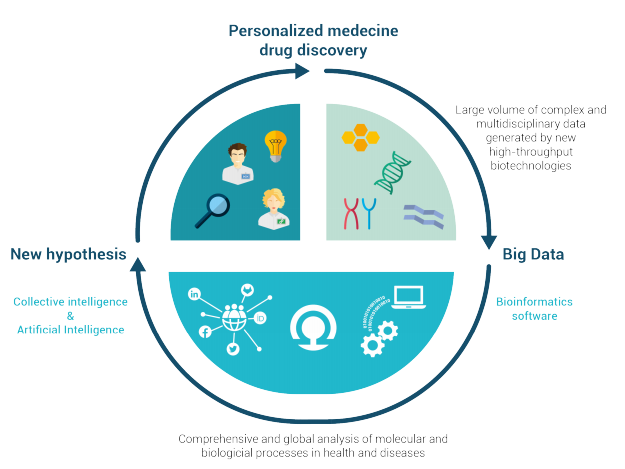
\includegraphics[width=0.7\textwidth]{poglavlja/1/slike/Primena.png}
\end{figure} 

Bioinformatika je spoj više različitih disciplina, kao što su:
\begin{itemize}
	\item Statistika
	\item Istraživanje podataka	
	\item Računarstvo
	\item Računarska biologija
	\item Biologija
	\item Biostatistika
\end{itemize}
Prikaz preklapanja ovih disciplina možemo videti na slici 1.2.
\begin{figure}[h]
\caption{Preklapanjem različitih disciplina dobijamo bioinformatiku.}
\centering
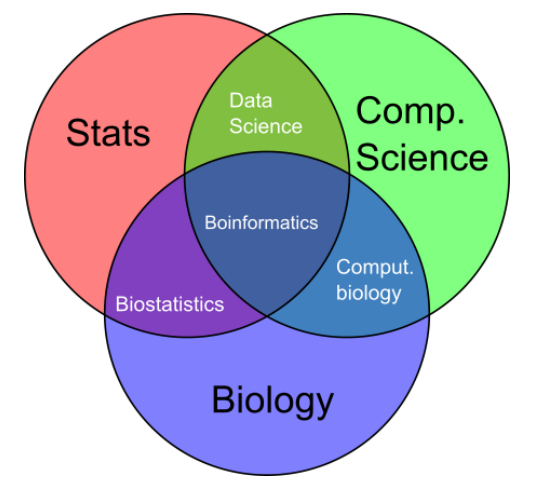
\includegraphics[width=0.7\textwidth]{poglavlja/1/slike/Multidisciplinarnost.png}
\end{figure}  

\newpage

\section{Replikacija genoma}
\label{sec:replikacija}

\subsection{DNK}

Dezoksiribonukleinska kiselina (akronimi DNK ili DNA, od engl. \textit{ deoxyribonucleic acid}), nukleinska kiselina koja sadrži uputstva za razvoj i pravilno funkcionisanje svih živih organizama. Zajedno sa RNK i proteinima, DNK je jedan od tri glavna tipa makromolekula koji su esencijalni za sve poznate forme života. \\\\
Sva živa bića svoj genetički materijal nose u obliku DNK, sa izuzetkom nekih virusa koji imaju ribonukleinsku kiselinu (RNK). DNK ima veoma važnu ulogu ne samo u prenosu genetičkih informacija sa jedne na drugu generaciju, već sadrži i uputstva za građenje neophodnih ćelijskih organela, proteina i RNK molekula. DNK segment koji sadrži ova važna uputstva se naziva gen.\\\\

DNK se sastoji iz dva polimerna lanca koji imaju antiparalelnu orijentaciju, i svaki od njih je sastavljen od azotnih baza:
\begin{itemize}
	\item adenin (A)
	\item timin (T)
	\item guanin (G)
	\item citozin (C)
\end{itemize}

\begin{figure}[h]
\caption{Prikaz DNK, slika preuzeta sa https://ghr.nlm.nih.gov/primer/basics/dna}
\centering
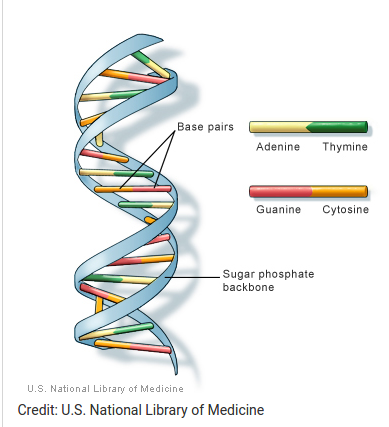
\includegraphics[width=0.5\textwidth]{poglavlja/1/slike/DNK.png}
\end{figure} 

Lanci DNK su međusobno spojeni i to tako da se veze uspostavljaju isključivo između adenina i citozina ili između guanina i timina. Na osnovu toga, ako nam je poznat sastav jednog lanca, lako možemo zakljuciti i sastav drugog lanca, zbog čega se kaže da su DNK lanci \textbf{međusobno komplementarni}.\\\\
Da bismo lakše manipulisali sa informacijama koje DNK nosi i približili sadržaj računarskoj struci, DNK ćemo posmatrati kao nisku nad azbukom \textit{A,C,G,T}.

\subsection{Replikacija genoma u ćeliji}
Replikacija genoma je jedan od najvažnijih zadataka ćelije. Pre nego što se podeli, ćelija mora da najpre replicira svoj genom, tako da svaka od ćerki ćelija dobije svoju kopiju. \\\\
Dzejms Votson (engl. \textit{James Watson}) i Fransis Krik (engl. \textit{Fransis Crick}) su 1953. godine napisali rad u kome su primetili da postoji mehanizam za kopiranje genetskog materijala. Oni su uočili da se lanci roditeljskog DNK molekula odvijaju tokom replikacije i da se, potom, svaki lanac ponaša kao uzorak za sintezu novog lanca (na osnovu toga što se uvek spajaju iste aminokiseline A-C i G-T, rekreiranje lanca je moguće). Kao rezultat ovakvog ponašanja, proces replikacije počinje parom komplementarnih lanca i završava se sa dva para komplementarnih lanaca, kao što se može videti na slici ispod.\\\\

\begin{figure}[h]
\caption{Prikaz replikacije}
\centering
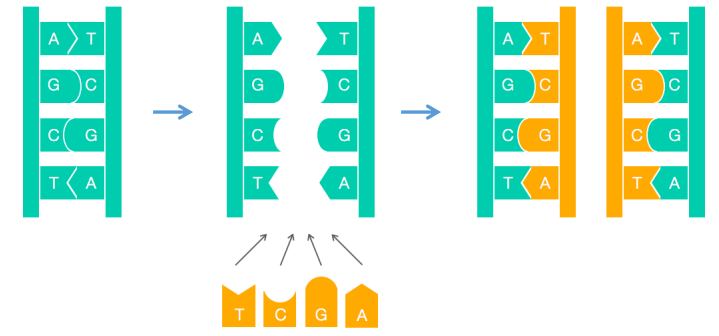
\includegraphics[width=1\textwidth]{poglavlja/1/slike/Replikacija.png}
\end{figure} 

Replikacija počinje u regionu genoma koji se naziva \textbf{početni region replikacije} (skraćeno \textit{oriC}), izvode je enzimi koje se nazivaju DNK polimeraze, koje predstavljaju mašine za kopiranje na molekularnom nivou.\\\\
Nalaženje početnog regiona replikacije predstavlja veoma važan problem, ne samo za razumevanje funkcionisanja kako se ćelije repliciraju, već je koristan i u raznim biomedicinskim problemima. Na primer, neki metodi genskih terapija uključuju genetski izmenjene mini genome, koji se zovu virusni vektori, zbog svoje sposobnosti da prodru kroz ćelijski zid (poput pravih virusa). Virusni vektori u sebi nose veštačke gene koji unapredjuju postojeći genom. Genska terapija je prvi put uspešno izvršena 1990. godine na devojčici koja je bila toliko otporna na infekcije da je bila primorana da živi isključivo u sterilnom okruženju.\\\\
Osnovna ideja genske terapije je da se pacijent, koji pati od nedostatka nekog bitnog gena, zarazi viralnim vektorom koji sadrži veštački gen koji enkodira terapeutski protein. Jednom kad je unutar ćelije, vektor se replicira, što dovodi do lečenja bolesti pacijenta. Da bi moglo da dodje do ovoga, biolozima je neophodno da znaju gde je \textit{oriC}.

\subsubsection{Kako ćelija prepoznaje \textit{oriC}?}
Pitamo se kako ćelija prepoznaje oriC? Sigurno je da postoji neka niska aminokiselina koja označava oriC, ali kako ga prepoznati?\\\\
Ograničimo se na bakterijski genom, koji se sastoji od jednog kružnog hromozoma. Istraživanje je pokazalo da je region, koji predstavlja oriC kod bakterija,
dug svega nekoliko stotina nukleotida.\\\\

\begin{figure}[h]
\caption{Prikaz početka replikacije kod bakterija}
\centering
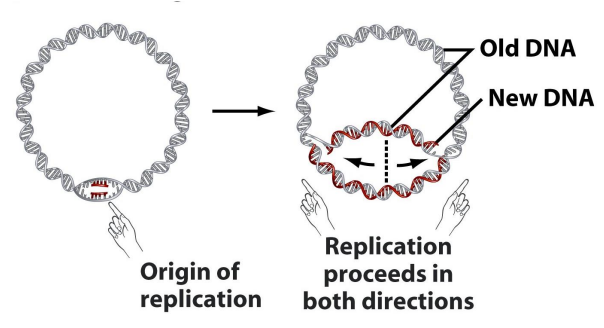
\includegraphics[width=0.7\textwidth]{poglavlja/1/slike/Replikacija_bakterija.png}
\end{figure} 

Poznato je da DNKA utiče na početak replikacije. \textit{DNKA} je protein koji se vezuje na kratki segment unutar oriC, poznatiji kao \textbf{DNKA boks}. Ona predstavlja poruku unutar sekvence DNK koja govori proteinu DNKA da se veže baš tu. Postavlja se pitanje kao pronaći taj region bez prethodnog poznavanja izgleda DNKA boks? \\\\

Da bismo bolje razumeli \textit{problem skrivene poruke} uzmimo za primer priču Edgara Alana Poa - $"$Zlatni jelenak$"$ (engl. \textit{$"$The Gold-Bug$"$}).
Naime, u toj priči jedan od likova, Vilijam Legrand (engl. \textit{William Legrand}), treba da dešifruje poruku :\\

\texttt{53++!305))6*;4826)4+.)4+);806*;48!8`6
0))85;]8*:+*8!83(88)5*!;46(;88*96*?;8\\
)*+(;485);5*!2:*+(;4956*2(5*4)8`8*;40
69285);)6!8)4++;1(+9;48081;8:8+1;48!8
5;4)\\485!528806*81(+9;48;(88;4(+?34;48
)4+;161;:188;+?;}\\\\
On uočava da se $"$;48$"$ pojavljuje veoma često, i da verovatno predstavlja $"$THE$"$, najčešću reč u engleskom jeziku. Znajući to, zamenjuje karaktere odgovarajućim slovima i postepeno dešifruje celu poruku.\\\\
\texttt{53++!305))6*THE26)H+.)H+)806*THE
!E`60))E5;]E*:+*E!E3(EE)5*!TH6(T
EE*96*?;E)*+\\(THE5)T5*!2:*+(TH956
*2(5*H)E`E*TH0692E5)T)6!E)H++T1(
+9THE0E1TE:E+1\\THE!E5T4)HE5!52880
6*E1(+9THET(EETH(+?34THE)H+T161T
:1EET+?T}\\\\
Želeli bismo da ovaj princip primenimo na naš problem nalaska \textit{oriC}-a. Ideja je da uvidimo da li postoje reči koje se neuobičajeno često pojavljuju. Uvedimo termin k-gram da označimo string dužine $k$ i COUNT(Text, Pattern) da označimo broj puta kojih se k-gram $Pattern$ pojavio u tekstu $Text$. Osnovna ideja je da pomeramo prozor, iste dužine kao k-gram $Pattern$, niz tekst, usput proveravajući da li se pojavljuje $Pattern$ u nekome od njih. 

\begin{lstlisting}
PATTERNCOUNT(Text, Pattern)
	count = 0
	for i = 0 to |Text| - |Pattern|
		if Text(i,|Pattern|) = Pattern
			count = count + 1 
	return count
\end{lstlisting}
	
Za neki $Pattern$ kažemo da je on \textit{najčešći k-gram} u tekstu $Text$, ako je njegov $COUNT$ najveći među svim k-gramima. Na primer, \textbf{ACTAT} je najčešći 5-gram u tekstu $Text$ = ACA\textbf{ACTAT}GCA\textbf{ACTAT}CGGGACA\textbf{ACTAT}CCT, a \textbf{ATA} je najčešći 3-gram u $Text$ = CG\textbf{ATATA}TCC\textbf{ATA}G.\\\\
Sada, problem pronalaska čestih reči možemo posmatrati kao računarski problem:\\
\begin{tcolorbox}
\textbf{Problem čestih reči:} Pronaći najčešće k-grame u niski karaktera.\\
\textit{Ulaz:} Niska Text i ceo broj k.\\
\textit{Izlaz:} Svi najčešći k-grami u niski Text. \\\\
\end{tcolorbox}
Osnovni algoritam za pronalazak čestih k-grama u stringu $Text$ proverava sve k-grame koji se pojavljuju u tom stringu (takvih k-grama ima $|Text|-k+1$) i potom izračunava koliko puta se svaki k-gram pojavljuje. Da bismo implementirali ovaj algoritam, moramo da izgenerišemo niz $COUNT$, gde je $COUNT(i) = COUNT(Text, Pattern)$ za $Pattern = Text(i,k)$.\\

\begin{lstlisting}
FrequentWords(Text, k)
	FrequentPatterns <- an empty set
	for i = 0 to |Text| - k
		Pattern <- the k-mer Text(i,k)
		COUNT(i) <- PatternCount(Text, Pattern)
	maxCount <- max value in array COUNT
	for i = 0 to |Text| - k
		if COUNT(i) = maxCount
			add Text(i,k) to FrequentPatterns
	remove duplicates from FrequentPatterns
	return FrequentPatterns
\end{lstlisting}

Pitamo se, sada, kolika je složenost ovakvog pristupa?\\
Ovaj algoritam, iako uspešno nalazi ono što se od njega traži, nije najefikasniji. S obzirom na to da svaki k-gram zahteva $|Text|-k+1$ provera, svaki od njih zahteva i do $k$ poređenja, pa je broj koraka izvršavanja funkcije $PatternCount(Text, Pattern)$ zapravo $(|Text|-k+1)*k$. Osim toga, $FrequentWords$ mora pozvati $PatternCount$ $|Text|-k+1$ puta (po jednom za svaki k-gram teksta), tako da je ukupan broj koraka \textit{$(|Text|-k+1)*(|Text|-k+1)*k$}.\\Iz navedenog, možemo zaključiti da je ukupna cena izvršavanja algoritma $FrequentWords$ \textbf{$O(|Text|^2*k)$}.

\subsubsection{Primer: Pronalazak čestih reči kod bakterije \textit{Vibrio cholerae}} 

Posmatrajmo, najpre, tablicu najčešćih k-grama u \textit{oriC} regionu bakterije \textit{Vibrio cholerae}. Da li nam se čini da se neki k-grami pojavljuju neuobičajeno često?\\ 

\begin{figure}[h]
\caption{Tablica najčešćih k-grama u \textit{oriC} regionu bakterije Vibrio cholerae}
\centering
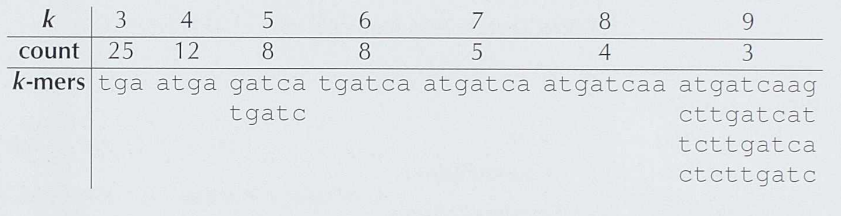
\includegraphics[width=1\textwidth]{poglavlja/1/slike/Tablica_VC.png}
\end{figure} 

Na primer, 9-gram \textbf{ATGATCAAG} se pojavljuje tri puta u \textit{oriC} regionu, da li nas to iznenađuje?\\

\begin{figure}[h]
\caption{Prikaz 9-grama ATGATCAAG i njegovog komplementa u \textit{oriC} regionu Vibrio cholerae}
\centering
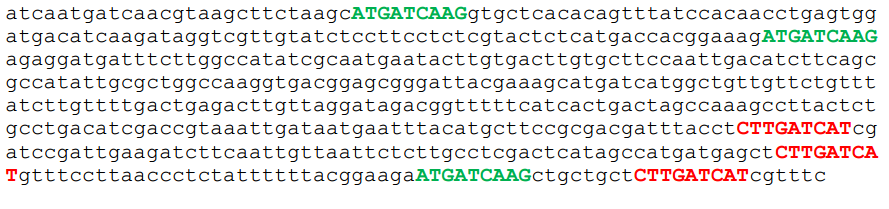
\includegraphics[width=1\textwidth]{poglavlja/1/slike/9_VC.png}
\end{figure} 

Označili smo najčešće 9-grame, umesto nekih drugih k-grama, jer je eksperimentima pokazano da su DNKA boksovi kod bakterija dugi 9 nukleotida. Verovatnoća da postoji 9-gram koji se pojavljuje 3 ili više puta u proizvoljno generisanom DNK stringu dužine 500 je $1/1300$. Uočimo da postoje četiri različita 9-grama koji se ponavljaju tri ili više puta u ovom regionu, to su: ATGATCAAG, CTTGATCAT, TCTTGATCA i CTCTTGATC.\\\\

Mala verovatnoća da se neki 9-gram toliko puta pojavi u \textit{oriC}-u kolere, govori nam da neki od četiri 9-grama koje smo pronašli može biti potencijalni DNKA boks, koji započinje replikaciju. Ali, koji?\\\\

Podsetimo se da nukleotidi A i T, kao i C i G, su komplementarni. Ako imamo jednu stranu lanca DNK i neke slobodne nukleotide, možemo lako zamisliti sintezu komplementarnog lanca, kao što se vidi na slici ispod. 

\begin{figure}[h]
\caption{Komplementarni lanci se $"$kreću$"$ u suprotnim smerovima.}
\centering
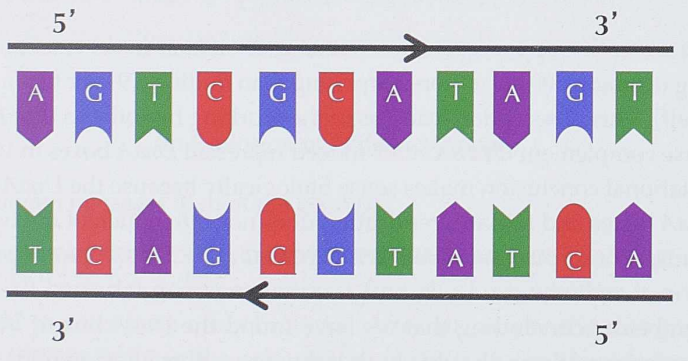
\includegraphics[width=1\textwidth]{poglavlja/1/slike/Komplementarni.png}
\end{figure} 

Posmatrajmo ponovo sliku 1.7. Na njoj možemo uočiti 6 pojavljivanja niski ATGATCAAG i CTTGATCAT, koji su zapravo komplementarni. Naći 9-gram koji se pojavljuje 6 puta u DNK nisci dužine 500 nukleotida, je još više iznenadjujuće, nego pronaći 9-gram koji se pojavljuje tri puta. Ovo posmatranje nas dovodi do toga da je ATGATCAAG (zajedno sa svojim komplementom) zaista DNKA boks Vibrio cholerae. Ovaj zaključak ima i smisla biološki, jer DNKA proteinu, koji se vezuje i započinje replikaciju, nije bitno za koji od dva lanca se vezuje.\\\\

\subsubsection{Primer: Pronalazak čestih reči kod bakterije \textit{Thermotoga petrophila}} 

Nakon što smo pronašli skrivenu poruku za Vibrio cholerae, ne bi trebalo da odmah zaključimo da je ta poruka ista kod svih bakterija. Najpre bi trebalo da proverimo da li se ona nalazi u \textit{oriC} regionu drugih bakterija, možda različite bakterije, imaju drugačije DNKA boksove. Uzmimo, za primer, \textit{oriC} region bakterije Thermotoga petrophila. Ona predstavlja bakteriju koja obitava u izrazito toplim regionima, na primer u vodi ispod rezervi nafte, gde temperature prelaze 80 stepeni Celzijusa. Pogledajmo kako izgleda \textit{oriC} region ove bakterije.

\begin{figure}[h]
\caption{Prikaz \textit{oriC} regiona Thermotoga petrophila}
\centering
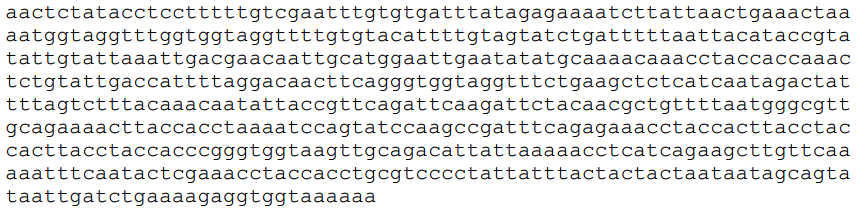
\includegraphics[width=1\textwidth]{poglavlja/1/slike/OriC_TP.png}
\end{figure} 

Možemo lako uočiti da se u ovom regionu nigde ne javljaju niske ATGATCAAG ili CTTGATCAT, iz čega zaključujemo da različite bakterije mogu koristiti različite DNKA boksove, kako bi pružile skrivenu poruku DNKA proteinu. Odnosno, za različite genome imamo različite DNKA boksove.

Najčešće reči u ovom \textit{oriC} su:
\begin{itemize}
	\item AACCTACCA, 
	\item ACCTACCAC,
	\item GGTAGGTTT,
	\item TGGTAGGTT,
	\item AAACCTACC,
	\item CCTACCACC
\end{itemize}

Pomoću alata koji se zove Ori-Finder, nalazimo CCTACCACC i njegov komplement GGTGGTAGG kao potencijalne DNKA boksove naše bakterije. Ove dve niske se pojavljuju ukupno 5 puta.

\begin{figure}[h]
\caption{Prikaz CCTACCACC i njenog komplementa u \textit{oriC} regionu Thermotoga petrophila}
\centering
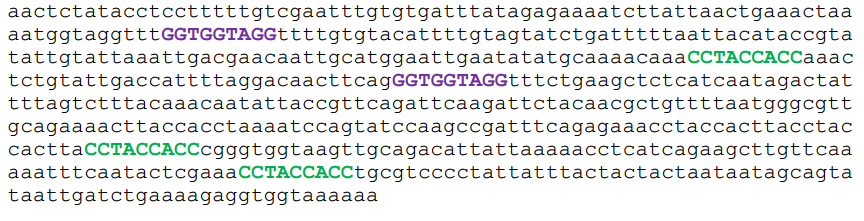
\includegraphics[width=1\textwidth]{poglavlja/1/slike/TP.png}
\end{figure} 
Naučili smo da pronađemo skrivene poruke ako je \textit{oriC}
dat, ali ne znamo da pronađemo \textit{oriC} u genomu.

\subsection{Pronalaženje početnog regiona replikacije}

Zamislimo da pokušavamo da nađemo \textit{oriC} u novom sekvenciranom genomu bakterije. Ako bismo tražili niske poput ATGATCAAG/CTTGATCAT ili CCTACCACC/GGTGGTAGG to nam verovatno ne bi bilo puno od pomoći, jer novi genom može koristiti potpuno drugačiju skrivenu poruku. Posmatrajmo, zato, drugačiji problem: umesto da tražimo grupe određenog k-grama, pokušajmo da nađemo svaki k-gram koji formira grupu u genomu. Nadajmo se da će nam lokacije ovih grupa u genomu pomoći da odredimo lokaciju \textit{oriC}-a.\\Ideja je da pomeramo prozor fiksirane dužine L kroz genom, tražeći region u kome se k-gram pojavljuje više puta uzastopno. Za L ćemo uzeti vrednost 500, koja predstavlja najčešću dužinu \textit{oriC}-a kod bakterija. \\\\
Definisali smo k-gram kao \textit{grupu}, ako se pojavljuje više puta unutar kratkog intervala u genomu. Formalno, k-gram Pattern formira (L, t) grupu unutar niske Genome ako postoji interval genoma, dužine L, u kome se k-gram pojavljuje barem t puta. \\\\
\begin{tcolorbox}
\textbf{Problem pronalaženja grupa.} Naći k-grame koji
formiraju grupe unutar niske karaktera.\\
Ulaz. Niska Genome i celi brojevi k (dužina
podniske), L (dužina prozora) i t (broj podniski u
grupi).\\
Izlaz. Svi k-grami koji formiraju (L, t)-grupe u
niski Genome.
\end{tcolorbox}

U genomu bakterije E.coli postoji 1904 različitih 9-
grama koji formiraju (500,3)-grupe. Koji od njih
ukazuje na početni region replikacije?

\subsubsection{Iskrivljeni dijagrami}

S obzirom na to da imamo veliku količinu statističkih podataka, pitamo se kako ih možemo upotrebiti da bismo došli do lokacije \textit{oriC}-a? U tome nam mogu pomoći \textbf{iskrivljeni dijagrami}(engl. \textit{skew diagram}). Osnovna ideja je da prođemo kroz genom i da računamo razliku između količine guanina(G) i citozina(C). Ako ova razlika raste, onda možemo pretpostaviti da se krećemo niz polulanac koji ide na desno (u nastavku samo polulanac, smer $5'-> 3'$), a ako razlika počne da se smanjuje, onda pretpostavljamo da smo na obrnutom polulancu ($3' -> 5'$). Zbog procesa koji se naziva deaminacija (gubljenje aminokiselina), svaki polulanac ima manjak citozina u poređenju sa guaninom, a svaki obrnuti polulanac ima manjak guanina u odnosu na citozin. 

\begin{figure}[h]
\caption{Prikaz kretanja.}
\centering
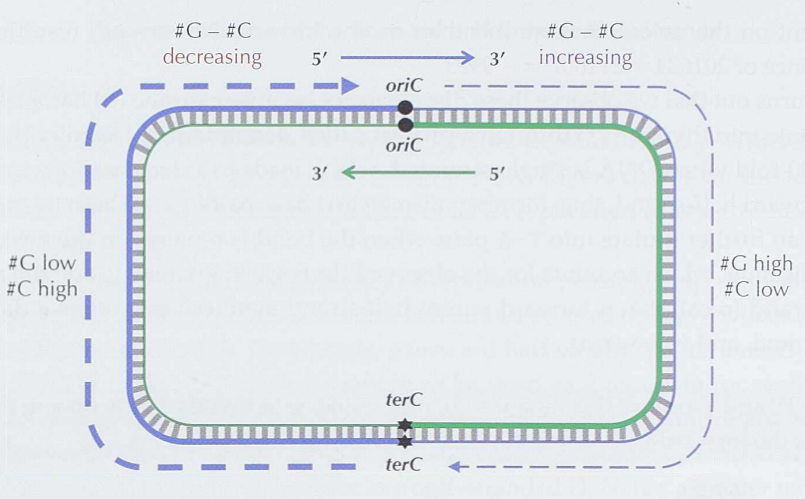
\includegraphics[width=1\textwidth]{poglavlja/1/slike/Polulanci_CG.png}
\end{figure} 

\begin{figure}[h]
\caption{Iskrivljeni dijagram genoma Genome = CATGGGCATCGGCCATACGCC.}
\centering
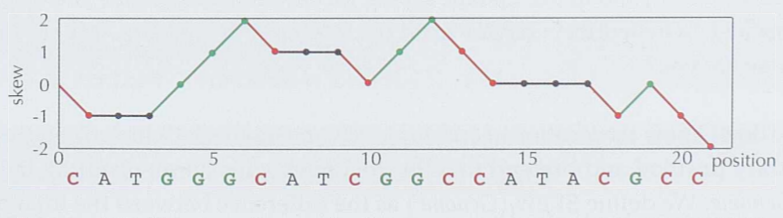
\includegraphics[width=1\textwidth]{poglavlja/1/slike/skew.png}
\end{figure} 

Posmatrajmo iskrivljeni dijagram bakterije Ešerihija Koli. Lako uočavamo minimalnu vrednost skew dijagrama.

\begin{figure}[h]
\caption{Iskrivljeni dijagram Ešerihije koli.}
\centering
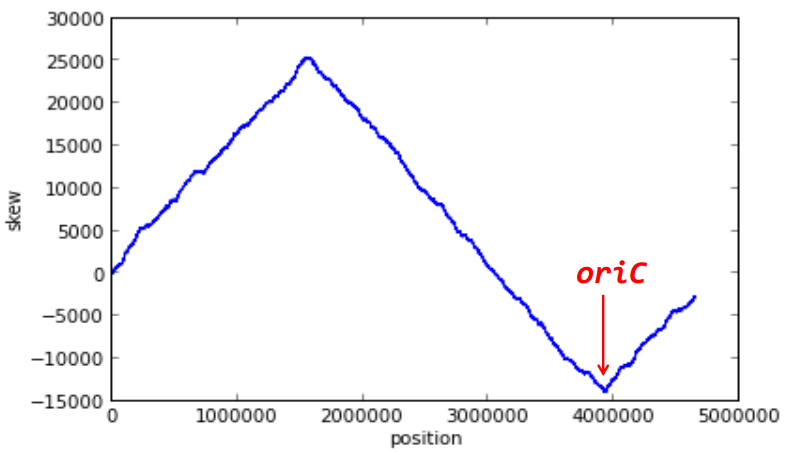
\includegraphics[width=1\textwidth]{poglavlja/1/slike/Ecoli_oriC.png}
\end{figure} 

Minimalna vrednost iz iskrivljenog dijagrama ukazuje baš na ovaj region:

\begin{figure}[H]
\caption{Region na koji pokazuje minimalna vrednost iskrivljenog dijagrama Ešerihije koli.}
\centering
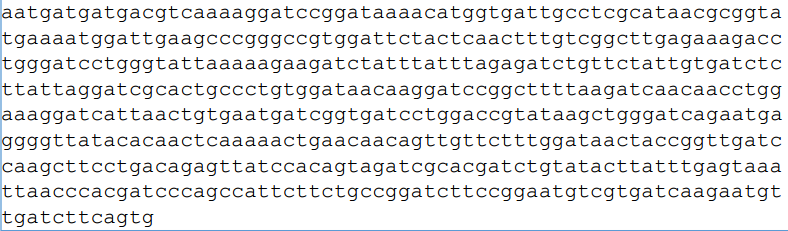
\includegraphics[width=1\textwidth]{poglavlja/1/slike/ecoli_region.png}
\end{figure} 

Uočimo da u ovom regionu nema čestih 9-grama (koji se pojavljuju 3 ili više puta). Iz toga zaključujemo da, iako smo uspeli da nađemo \textit{oriC} bakterije Ešerihija koli, nismo uspeli da nađemo DNKA boksove. Međutim, pre nego što odustanemo od potrage, osmotrimo još jednom \textit{oriC} Vibrio colerae, kako bismo pokušali da nađemo način da izmenimo naš algoritam i uspemo da lociramo DNKA boksove u Ešerihiji koli. Veoma brzo, može se uvideti da osim tri pojavljivanja ATGATCAAG i tri pojavljivanja CTTGATCAT, \textit{oriC} Vibrio cholerae sadrži i dodatna pojavljivanja ATGATCAAC i CATGATCAT koji se razlikuju samo u jednom nukleotidu od gornjih niski. Ovo još više povećava šanse da smo naišli na prave DNKA boksove, a ima i biološkog smisla. Naime, DNKA se može vezati i za nesavršene DNKA boksove, one koji se razlikuju u nekoliko nukleotida.\\\\


\begin{figure}[H]
\caption{Prikaz pojavljivanja nesavršenih niski nukleotida.}
\centering
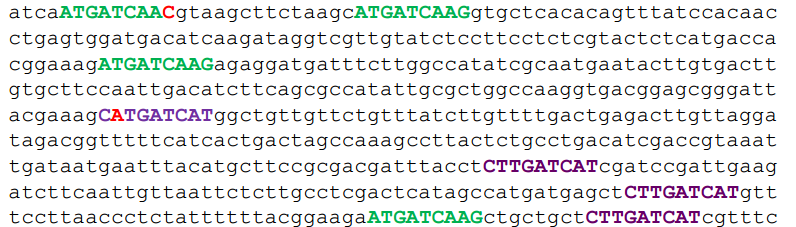
\includegraphics[width=1\textwidth]{poglavlja/1/slike/nesavrseni1.png}
\end{figure} 

Cilj nam je da sada izmenimo algoritam čestih reči (FrequentWords) tako da možemo da pronađemo DNKA boksove koji su predstavljeni čestim k-gramima, sa mogućim izmenama na pojedinim nukleotidima. Ovaj problem nazvaćemo problem čestih reči sa propustima.\\\\
\begin{tcolorbox}
\textbf{Problem čestih reči sa propustima.} Pronaći najčešće k-grame sa
propustima u niski karaktera.\\
Ulaz: Niska Text i celi brojevi k i d.\\
Izlaz: Svi najčešći k-grami sa najviše d propusta u niski Text. \\
\end{tcolorbox}
Pokušajmo, još jednom, sa pronalaskom DNKA boksova kod Ešerihije koli, tako što ćemo naći najčešće 9-grame sa propustima i komplementima u regionu \textit{oriC} koji nam je predložen minimalnom vrednošću iskrivljenog dijagrama. Pokušaćemo sa malim prozorom koji ili počinje ili se završava ili je centriran na poziciji najmanje iskrivljenosti. Ovakvim izvođenjem pronalazimo TTATCCACA/TGTGGATAA kao najčešći 9-gram. Međutim, ovo nije jedini 9-gram. Za ostale 9-grame još uvek ne znamo čemu služe, ali znamo da nose skrivene informacije, da se grupišu unutar genoma i da većina njih nema veze sa replikacijom. 

\begin{figure}[H]
\caption{Prikaz pronađenih niski sa propustima i komplementima u \textit{oriC} regionu Ešerihije koli.}
\centering
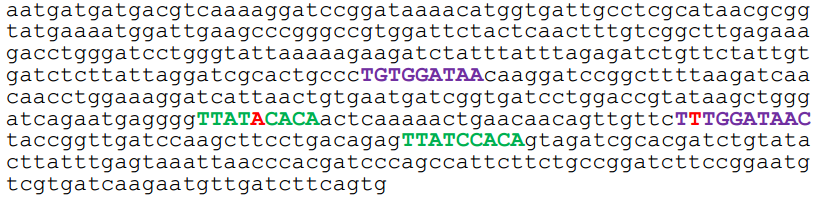
\includegraphics[width=1\textwidth]{poglavlja/1/slike/ecoli_poslednji.png}
\end{figure} 

\newpage

\section{Zadaci sa vežbi}
U nastavku će biti predstavljeni zadaci sa vežbi na kursu rađeni u programskom jeziku Python.

\subsection{FrequentWords}

\lstinputlisting[language=Python]{poglavlja/1/kodovi/1.py}

\subsection{Faster FrequentWords}

\lstinputlisting[language=Python]{poglavlja/1/kodovi/3.py}

\subsection{Skew Diagram}

\lstinputlisting[language=Python]{poglavlja/1/kodovi/4.py}

\subsection{FrequentWords With Mismatches}

\lstinputlisting[language=Python]{poglavlja/1/kodovi/5.py}


\chapter{Kako složiti genomsku slagalicu od milion delova?}

\section{Šta je sekvenciranje genoma?}

Sa biološke strane, genom jednog organizma predstavlja njegov genetski materijal. Kod većine organizama, genetski materijal je sadržan u DNK. Kod čoveka, genom sadrži oko tri milijarde nukleotida. Genomi nekih organizama su i 100 puta veći od humanog genoma. 

Sa računarske strane, genom je niska karaktera nad azbukom $\{A, C, G, T\}$.

% nije mi jasan veliki razmak koji se napravi  u tekstu na ovom mestu xD

\subsection{Kratka istorija sekvenciranja genoma}

1977. godine Walter Gilbert i Frederick Sanger razvijaju nezavisne metode sa sekvenciranje DNK, za koje su, 1098. godine, podelili su Nobelovu nagradu.
Njihove metode za sekvenciranje su bile veoma skupe - 3 milijarde dolara za sekvenciranje humanog genoma.
\\
\\
Krajem 2000-tih Sanger metodom je sekvencioniran veliki broj genoma. Visoka cena je bila ograničavajući faktor i za dalji napredak je bila neophodna nova tehnologija sekvencioniranja.
\\
\\
\textbf{NGS} predstavlja metode nove generacije sekvencioniranja. Krajem 2000-tih, na tržištu se pojavljuju nove mašine za sekvenciranje. \textit{Illumina} smanjuje trošak sekvencioniranja humanog gemona sa 3 milijarde na 10 hiljada dolara. Kompanija \textit{Complete Genomics} otvara genomsku fabriku u Silikonskoj dolini koja sekvencionira stotine genoma mesečno.
Pekinški genomski institut (BGI - Beijing Genome Institute) preuzima Complete Genomics 2013. godine i postaje najveći svetski centar za sekvenciranje genoma.
Na slici \ref{slika:cena} prikazano je kako se cena sekvencioniranja menjala godinama.


\begin{figure}[H]
	\centering
	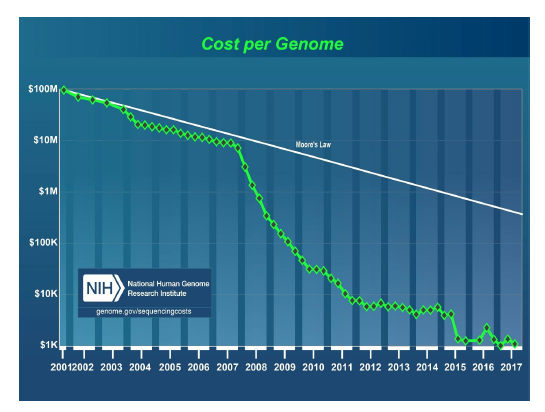
\includegraphics[width=1\textwidth]{poglavlja/3/slike/cena_sekvencioniranja.png}
	\caption{Cena sekvencioniranja kroz istoriju.}
	\label{slika:cena}
\end{figure} 



\subsection{Sekvenciranje ličnih genoma}

Genomi se kod različitih ljudi razlikuju na malom broju pozicija (u proseku sadrže jednu mutaciju na hiljadu nukleotida). Ova razlika je odgovorna za različite visine kod ljudi, da li će imati sklonost ka visokom holesterolu ili ne, za veliki broj genetskih bolesti, itd.
\\
\\
2010: Nicholas Volker je postao prvo ljudsko biće čiji je život spašen zahvaljujući genomskom sekvencioniranju.
Lekari nisu mogli da postave tačnu dijagnozu i morali su da ga podvrgnu velikom broju operacija pokušavajući da je utvrde. Sekvenciranje je otkrilo retku mutaciju na jednom genu (XIAP) koja je bila povezana sa oštećenjem njegovog imunog sistema. Ovo otkriće je navelo lekare na adekvatnu terapiju koja je rešila problem.

\section{Eksplozija u štampariji}

Zamislite da imamo hiljadu kopija istog izdanja novina na jednoj gomili, a ispod njih postavljen je dinamit. Upalimo fitilj i zamislimo da nije sve samo izgorelo već da se raspršilo u milione delića papira. Kako možemo da iskoristimo te deliće da bismo saznali koje su bile vesti iz tog izdanja? Ovaj problem nazvaćemo \textbf{Problem novina} (\ref{slika:eksplozija}). 

\begin{figure}[H]
	\centering
	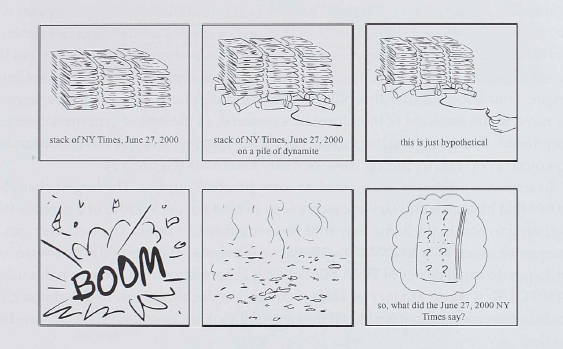
\includegraphics[width=1\textwidth]{poglavlja/3/slike/eksplozija.png}
	\caption{Problem novina poslužiće nam u razumevalju problema slaganja genoma.}
	\label{slika:eksplozija}
\end{figure} 


Problem novina je mnogo teži nego što izgleda. Kako smo imali više kopija istog izdanja, i kako smo izgubili neki deo informacija prilikom eksplozije, ne možemo samo da prilepimo deliće novina kao da su slagalica. Umesto toga, potrebno je da preklopimo delove različitih novina kako bismo rekonstruisali jedan primerak.


\begin{figure}[H]
	\centering
	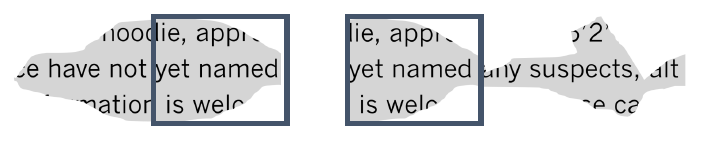
\includegraphics[width=1\textwidth]{poglavlja/3/slike/delici.png}
	\caption{Spajanje delova različitih novina koji se jednim delom preklapaju.}
	\label{slika:delici}
\end{figure} 


Kakve sad to veze ima sa našim problemom? Određivanje redosleda nukleotida u genomu, odnosno sekvenciranje genoma, predstavlja bitan problem u bioinformatici. Dužine genoma variraju: humani genom je dugačak oko 3 milijarde nukleotida, dok je genom jendoćelijskog organizma Amoeba dubia čak 200 puta duži. 


Moderne mašine za sekvenciranje (sekvenceri) ne mogu da pročitaju ceo genom nukleotid po nukleotid od početka do kraja (kao što bismo pročitali knjigu).
Mogu samo da iseckaju genom i generišu njegova kratka očitavanja. Kako to zapravo funkcioniše (\ref{slika:sekvenciranje})? Sekvencer dobija milione kopija istog genoma. Zatim vrši očitavanja čime dobijamo deliće odnosno kratke podniske. Neki delovi odnosno očitavanja biće izgubljena (kao delići novina u eksploziji, dakle gubimo deo informacija). Očitavanja su izmešana i ono što nam sekvencer daje je zapravo kolekcija podniski koje treba spojiti u jednu. Sastavljanje genoma nije isto kao i slaganje slagalice: moramo da koristimo preklapajuća očitavanja da bismo rekonstruisali genom.


\begin{figure}[H]
	\centering
	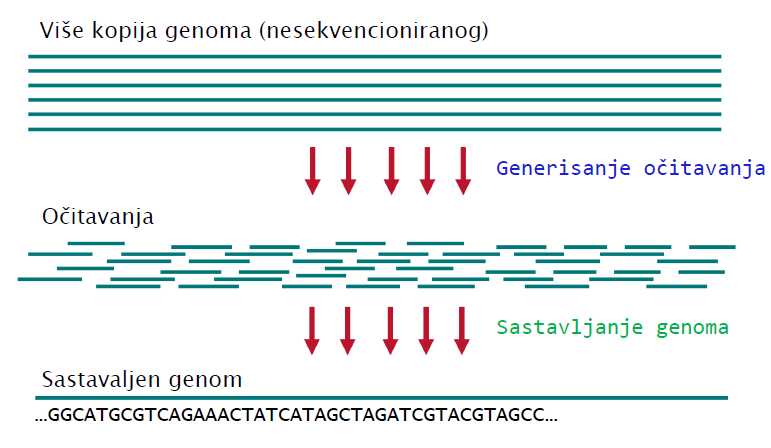
\includegraphics[width=1\textwidth]{poglavlja/3/slike/sekvencioniranje.png}
	\caption{Ilustracija problema.}
	\label{slika:sekvenciranje}
\end{figure} 


\section{Problem sekvenciranja genoma}

\begin{problem}
	[Problem sekvencioniranja genoma] Rekonstruisati genom na osnovu očitavanja.
	\\ Ulaz. Kolekcija niski Reads.
	\\ Izlaz. Niska Genome rekonstruisana na osnovu Reads.
\end{problem}

% ovo dopuniti sa snimka pošto nema ni u knjizi baš
Ovo nije dobro definisan problem. 


\subsection{k-gramski sastav niske}

k-gramski sastav niske $Text$ ($Composition_k(Text)$) predstavlja kolekcija podnsiki dužine $k$ niske $Text$, uključujući duplikate. Na primer:


% ovo sigurno može lepše xD (slajd 32)
\begin{align*}
	Composition_3(TAATGCCATGGGATGTT) =& \\
	TAA AAT ATG TGC GCC CCA CAT ATG TGG GGG GGA GAT ATG TGT GTT =& \\
	AAT ATG ATG ATG CAT CCA GAT GCC GGA GGG GTT TAA TGC TGG TGT
\end{align*}

Sada možemo malo bolje da definišemo problem.

\begin{problem}
	[Problem rekonstrukcije niske] Rekonstruisati nisku na osnovu njenog k-gramskog sastava.
	\\ Ulaz. Kolekcija k-grama.
	\\ Izlaz. Niska Genome takva da je $Composition_k(Genome)$ ekvivalentno kolekciji k-grama
\end{problem}


Naivni pristup ovom problemu bio bi da odaberemo jedan k-gram za početni. Zatim nižemo ostale tako da se sufiks poslednjeg odabranog poklopi sa prefiksom nekog od preostalih k-grama. Pri tome, ako ima više takvih k-grama, biramo jedan, bilo koji, Na ovaj način možemo doći do rešenja, ali je veoma skupo. Pri tome, velika je šansa da ćemo se negde zaglaviti (tj. nijedan od preostalih k-grama neće biti kandidat za nadovezivanje na tekuću nisku) ili zbog izbora početnog k-grama ili zbog izbora nekog od preostalih k-grama kada je postojalo više odgovarajućih. Sledeći primer ilustruje ovaj problem:

Neka nam je dat sledeći 3-gramski sastav: 
$$AAT ATG ATG ATG CAT CCA GAT GCC GGA GGG GTT TAA TGC TGG TGT$$

Treba rekonstruisati nisku koja ima takav sastav. Biramo početni 3-gram, neka to bude na primer $TAA$. Zatim na njega treba nadovezati 3-gram koji počinje njegovim sufiksom dužine 2, odnosno onaj 3-gram koji ima prefiks $AA$. U našem slučaju, postoji jedan takav 3-gram i njega nadovezujemo na tekuću nisku, tako da sada imamo $TAAT$. Zatim biramo 3-gram čiji je prefiks $AT$. Ovog puta imamo 3 kandidata, ali, na našu sreću, sva tri su isti 3-grami, $ATG$. U takvom slučaju nije bitno koji smo odabrali, jer su svi jednaki. Nadovezujemo ga na tekuću nisku i dobijamo $TAATG$. Tražimo 3-grame sa prefiksom $TG$, koji do sad nisu upotrebljeni. Ponovo pronalazimo 3 kandidata. Međutim, u ovom slučaju, svi kandidati predstavljaju različite 3-grame, a to su $TGC$, $TGG$ i $TGT$. Naivni pristup kaže da biramo jedan od njih, i recimo da smo odabrali $TGT$ i dobili nisku $TAATGT$. Sada nam je potrebam 3-gram sa prefiksom $GT$ i tu dolazi do zaglavljivanja! 
Imamo još 3-grama koji nisu iskorišćeni za rekonstrukciju niske, ali nijedan ne možemo da iskoristimo u ovom trenutku! U takvim situacijama treba se vratiti u nazad do koraka u kom je bilo više kandidata.


\section{Rekonstrukcija niske kao problem Hamiltonove putanje}

Videli smo da nam naivni pristup ne odgovara i moramo smisliti bolje rešenje. Mogli bismo da iskoristimo znanja iz teorije grafova za rešavanje ovakvog problema. U tom slučaju, prvi zadatak je da našu nisku predstavimo u vidu grafa.


\subsection{Genom kao putanja}

Vratimo se na prethodni primer. Dat nam je k-gramski sastav niske :
$$Composition_3(TAATGCCATGGGATGTT) =$$
$$ TAA AAT ATG TGC GCC CCA CAT ATG TGG GGG GGA GAT ATG TGT GTT$$

Njega treba predstaviti kao graf. Možemo da napravimo po jedan čvor za svaki od k-grama. Zatim, potrebne su nam grane koje će povezati te čvorove. Dvs čvora su povezana usmerenom granom ako izlazni čvor ima sufiks jednak prefiksu ulaznog čvora te grane, kao što je prikazano na slici \ref{slika:graf1}.

\begin{figure}[H]
	\centering
	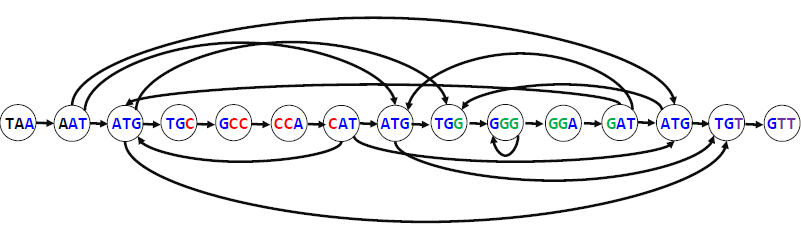
\includegraphics[width=1\textwidth]{poglavlja/3/slike/hamilton.png}
	\caption{Graf koji odgovara k-gramskom sastavu niske $TAATGCCATGGGATGTT$.}
	\label{slika:hamilton}
\end{figure} 

Jasno je da postoji više puteva u ovom grafu. Postavlja se pitanje, da li možemo da pronađemo genomsku putanju u ovom grafu, od svih koje postoje?

Podsetimo se šta je Hamiltonova putanja. Hamiltonova putanja je putanja koja posećuje svaki čvor u grafu tačno jednom. To je upravo ono što nam je potrebno za rešavanje problema. Svaki čvor predstavlja jedan k-gram i porebno nam je da svi k-grami budu uključeni u rekonstruisanu nisku tačno jednom.

\begin{problem}
	[Problem Hamiltonove putanje]
	Naći Hamiltonovu putanju u grafu.
	\\ Ulaz. Graf.
	\\Izlaz. Putanja koja posećuje svaki čvor u grafu tačno jednom.
\end{problem}

Iako deluje kao da smo rešili sve probleme, zapravo smo naišli na još jednu veliku prepreku. Naime, pronalaženje Hamiltonovog puta u grafu je NP-kompletan problem, što znači da ne postoji efikasan algoritam koji to radi.

U tom slučaju, moramo da se vratimo na početak, a to je predstavljanje k-gramskog sastava grafom.


\section{Rekonstrukcija niske kao Ojlerove putanje}


U prethodnoj sekciji k-grame smo predstavili čvorovima u grafu i u njemu tražili Hamiltonov put odnosno put koji obilazi svaki čvor tačno jednom. Videli smo da za taj problem još uvek nije poznat efikasan algoritam pa se sada pitamo kako možemo izmeniti graf tako da ne zahteva traženje Hamiltonove putanje.

Ono što se javlja kao ideja jeste obeležavanje grana umesto čvorova. Dakle, svaka grana biće obeležena jednim k-gramom, podniskama trih k-grama. Izlazni čvor biće obeležen prefiksom k-grama te grane, dok će ulazni čvor biti obeležen sufiksom istog tog k-grama. Na slici \ref{slika:ojler} ilustruje ovaj postupak za nisku $TAATGCCATGGGATGTT$.

\begin{figure}[H]
	\centering
	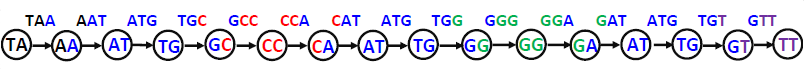
\includegraphics[width=1\textwidth]{poglavlja/3/slike/ojler.png}
	\caption{Graf koji odgovara 3-gramskom sastavu niske $TAATGCCATGGGATGTT$. Grane su obeležene 3-gramima, a čvorovi prefiksima/sufikisima.}
	\label{slika:ojler}
\end{figure} 


Primećujemo da su neki čvorovi obleženi identično (npr. imamo tri čvora sa oznakom $AT$). Sve čvorove koji imaju istu oznaku treba spojiti u jedan, pri čemu zadržavamo sve grane koje su ulazile u taj čvor ili su izlazile iz njega. Ponavljamo postupak dokle god imamo čvorove koji imaju istu oznaku i na kraju dobijamo graf koji nazivamo De Brojnov graf. 

\begin{figure}[H]
	\centering
	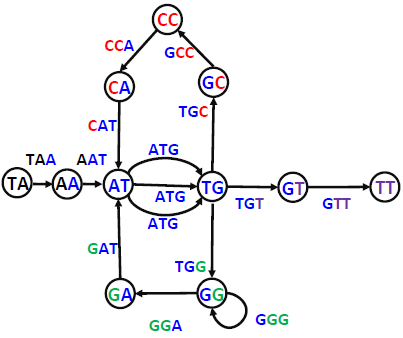
\includegraphics[width=0.6\textwidth]{poglavlja/3/slike/debrojnov.png}
	\caption{De Brojnov graf koji odgovara niski $TAATGCCATGGGATGTT$.}
	\label{slika:debrojnov}
\end{figure} 

Dobro, došli smo do nove reprezentacije niske pomoću grafa. Gde se sad nalazi naš \textit{Genome}? Kako nam se 3-grami sada nalaze na granama, a ne u čvorovima, potrebno je da pronađemo putanju u grafu koja prolazi sve grane tačno jednom. Takav put nazivamo \textit{Ojlerova putanja}. Srećom, algoritam za pronalaženje Ojlerove putanje u grafu nije NP-kompletan i možemo efikasno da je pronađemo.


\begin{problem}[Problem Ojlerove putanje]
	~\\ Pronaći Ojlerovu putanju u grafu.
	\\ Ulaz. Graf.
	\\ Izlaz. Putanja koja posećuje svaku granu u grafu tačno jednom.
\end{problem}


Sada znamo kako možemo da dobijemo nisku kada znamo de Brojnov graf koji odgovara njenom k-gramskom sastavu. Međutim, konstruisali smo de Brojnov graf na osnovu genoma, ali u realnim primenama, genom je nepoznat.


\section{De Brojnovi grafovi na osnovu kolekcije k-grama}

U redu, nije nam poznata niska, ali znamo njen k-gramski sastav. Za svaki k-gram pravimo dva čvora i jednu granu, na prethodno opisani način (\ref{slika:kgrami}).
Zatim lepimo identične čvorove sve dok ne dobijemo graf čiji svi čvorovi imaju različite oznake. Na slici je dat jedan korak ovog postupka, međutim tu nije kraj jer i dalje postoje čvorovi sa istim oznakama.

\begin{figure}[h]
	\centering
	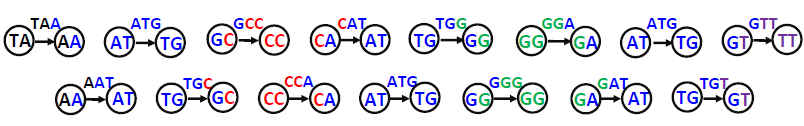
\includegraphics[width=1\textwidth]{poglavlja/3/slike/debrojnov1.png}
	\caption{Svaki k-gram prestavljen je pomoću dva čvora i jedne grane.}
	\label{slika:kgrami}
\end{figure} 

\begin{figure}[h]
	\centering
	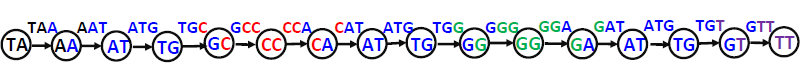
\includegraphics[width=1\textwidth]{poglavlja/3/slike/lepljenje.png}
	\caption{Postupak lepljenja čvorova. Posao nije završen!}
	\label{slika:lepljenje}
\end{figure} 


Po završetku postupka dobijamo de Brojnov graf koji je isti kao onaj koji smo dobili kada smo znali nisku. Svaka grana je označena jednim k-gramom. Svaki čvor je označen prefiksom/sufiksom izlazne/ulazne grane. Zalepljeni su svi čvorovi sa identičnim oznakama.

\section{Ojlerova teorema}

\begin{problem}[Problem Ojlerovog ciklusa]
	~\\ Pronaći ciklus Ojlerovom grafu.
	\\ Ulaz. Graf.
	\\ Izlaz. Ciklus koja posećuje svaku granu tačno jednom.
\end{problem}

\begin{teorema}[Ojlerova teorema]
	Svaki povezan graf i balansiran graf je Ojlerov.
\end{teorema}

Kažemo da je graf povezan ako za ma koja dva čvora postoji putanja koja ih povezuje.


%% MRAVI DOKAZUJU OJLEROVU TEOREMU

\begin{verbatim}
EulerianCycle(BalancedGraph)
form a Cycle by randomly walking in BalancedGraph (avoiding already visited edges)
while Cycle is not Eulerian
select a node newStart in Cycle with still unexplored outgoing edges
form a Cycle' by traversing Cycle from newStart and randomly walking afterwards
Cycle \leftarrow Cycle'
return Cycle
\end{verbatim}

\section{Sastavljanje parova očitavanja}

Od očitavanja do de Brojnovog grafa do genoma može se javiti više Ojlerovih putanja u grafu.

\subsection{DNK sekvenciranje sa parovima očitavanja} 

Imamo više identičnih kopija genoma i na slučajnim pozicijama sečemo genom na fragmente iste dužine \textit{InsertLength}. Zatim generišemo parove očitavanja: dva očitavanja sa krajeva svakog fragmenta na fiksiranoj udaljenosti.
Pod uparenim k-gramom podrazumevamo par k-grama na fiksiranom rastojanju d u genomu. Na primer, TCA i TCC na rastojanju d=11 čine jedan upareni k-gram.

\begin{problem} [Problem rekonstrukcije niske na osnovu parova očitavanja]
	~\\ Rekontruisati nisku na osnovu njenih uparenih k-grama.
	\\ Ulaz. Kolekcija uparenih k-grama.
	\\ Izlaz. Niska Text takva da je PairedComposition(Text) jednak kolekciji uparenih k-grama. 
\end{problem}

Kako konstruisati upareni de Brojnov graf na osnovu uparenog k-gramskog sastava?
Pretpostavimo da je dat genom (niska Genome). Posmatrajmo genom kao putanju u grafu obeleženom na osnovu njegovog uparenog kgramskog sastava.
\\
Pretpostavili smo da je dat genom (niska Genome). Posmatrali smo genom kao putanju u grafu obeleženom na osnovu njegovog uparenog k-gramskog sastava
\\
Sada pretpostavimo da nije dat genom već samo upareni k-gramski sastav

%% animacije, SVUDA ANIMACIJE!!!!!

~\\ Upareni de Brojnov graf na osnovu kolekcije uparenih k-grama:
\\ – Svaka grana je označena jednim uparenim k-gramom
\\ – Svaki čvor je označen prefiksima/sufiksima izlazne/ulazne grane
\\ – Zalepljeni su svi čvorovi sa identičnim oznakama.

\section{U realnosti}

Ovde smo imali neke nerealne pretpostavke.
\begin{itemize}
	\item  Savršena pokrivenost genoma očitavanjima (svaki k-gram iz genoma je očitan)
	\item Očitavanja ne sadrže greške
	\item Rastojanja između očitavanja u okviru parova očitavanja su egzaktna
	\item Nesavršena pokrivenost genoma očitavanjima (svaki k-gram iz genoma je očitan)
	\\ Očitavanja ne sadrže greške
	\\ Rastojanja između očitavanja u okviru parova očitavanja nisu egzaktna
\end{itemize}

\subsection{Savršena pokrivenost}

Prva nerealna pretpostavka je savršena pokrivenost.
\\
Očitavanja dužine 250 nukleotida dobijena Illumina tehnologijom predstavljaju samo mali deo 250-grama unutar genoma.
\\
Rešenje: razbiti dobijena očitavanja na kraće k-grame
\\
\\
Druga nerealna pretpostavka: očitavanja ne sadrže greške.

\newpage
\section{Zadaci sa vežbi}
U nastavku će biti predstavljeni zadaci sa vežbi na kursu rađeni u programskom jeziku Python.



\chapter{Kako sekvenciramo antibiotike?}
\setbookcodestyle


U ovom poglavlju i dalje govorimo o sekvenciranju, ali ćemo proširiti pogled i pokazati različite načine za sekvenciranje peptida. 

\section{Otkriće antibiotika} \label{otkrice}

Pre svega, krenućemo sa biološkim uvodom. Šta su to antibiotici? Sama reč antibiotik znači ,,onaj koji ubija život'', a tačnije, on predstavlja supstancu koja ubija bakterije. Kada ostavimo pomorandžu dugo negde gde je toplo, ona će da razvije čudne osobine kao što je buđ. Šta to znači? Buđ jeste jedna vrsta antibiotika što znači da se antibiotici nalaze u prirodi i da ih proizvode organizmi iz porodice gljiva (npr. buđi) i bakterija. 

Mi ćemo posmatrati antibiotike na molekularnom nivou koji nam govori od čega su oni zapravo izgrađeni. Od svih antibiotika posmatraćemo \textbf{\textit{tirocidin B1}}, antibiotik koji proizvodi bakterija \textit{Bacillus Brevis}. Tirocidin B1 na molekulskom nivou pripada \textit{peptidima}, kratkim niskama aminokiselina, odnosno malim proteinima. Ovo je skok u odnosu na ono što smo do sada posmatrali -- nukleotidne niske nad četvorostrukom azbukom $\Sigma = \{A, C, G, T\}$, odnosno DNK. Za DNK smo govorili da se pojavljuje u svakoj ćeliji svakog živog bića i da je veoma značajna supstanca jer sadrži recept (tačnije, nosi informaciju) za pravilno funkcionisanje i razvoj svakog živog bića. Da bi se svako živo biće pravilno razvijalo, neophodno je da njegove ćelije proizvode (sintetišu) u tačno određeno vreme određene supstance koje se nazivaju \textit{proteini}. DNK nosi informaciju o tome kako treba neki protein da izgleda, od čega treba da se sastoji. Zašto je to bitno? Na primer, kada je dan, neke biljke treba da vrše fotosintezu, a za vršenje fotosinteze treba u samim ćelijama biljaka da se sintetišu određeni proteini.

Proteini su, nakon nukleinskih kiselina, druga značajna grupa molekula koja sa računarske tačke gledišta takođe predstavlja dugačke niske, ali ne nad azbukom od 4 karaktera, nego nad azbukom od 20 karaktera, a svaki karakter predstavlja molekul koji se naziva \textit{aminokiselina}. Kao i nukleinske kiseline, aminokiseline se predstavljaju velikim latiničnim slovima $ \{V, K, L, F, P, W, N, Q, Y, G, A, I, M, D, E, S, T, C, R, H\}$, a pored toga postoje i troslovne oznake $\{Val, Lys, Leu, Phe, Pro, Trp, Asn, Gln, Tyr, Gly, Ala, Ile, Met, Asp, Glu, Ser, Thr, Cys, Arg, His\}$. U prirodi postoji mnogo više od 20 aminokiselina, ali 20 njih najčešće učestvuje u sastav proteina. DNK upravlja time kada će nastati protein u okviru ćelije. Recept za nastajanje svakog proteina je zapisan u DNK. Kako je taj recept zapisan, videćemo u nastavku.

Proteini se još nazivaju i \textit{polipeptidi}. Dužina proteina je obično od 100 aminokiselina do nekoliko hiljada (proteini su kraći od genomske sekvence). Tirocidin B1 je peptid jer se sastoji iz malog broja aminokiselina, svega deset -- $ V,K,L,F,P,W,F,N,Q,Y$. Problem sekvenciranja antibiotika jeste problem određivanja aminokiselina koje ulaze u sastav tog antibiotika. U prethodnom poglavlju smo sekvencirali genom, ali tehnike iz prethodnog poglavlja nećemo moći da koristimo u sekvenciranju tirocidina B1, što će biti objašnjeno u poglavlju \ref{pravljenje}.


\section{Kako bakterije prave antibiotike?} \label{pravljenje}

Pre rešavanja problema sekvenciranja antibiotika, govorićemo o zanimljivoj i kompleksnoj temi, a to je tema -- kako se prave proteini? Već je pomenuto da se u okviru DNK nalazi recept za pravljenje proteina. Sada je vreme da se zapitamo kako je sve to zapisano u DNK pomoću $A, C, G, T$.

Znamo da je DNK dvostruki lanac čiji su krajevi označeni sa 5' i 3' (uvek čitamo lanac od 5' ka 3'). DNK jeste jedna vrsta nukleinskih kiselina koje postoje u ćeliji živih bića. Pored nje, postoje i različite vrste \textbf{ribonukleinskih kiselinina}, odnosno \textbf{RNK}. Ribonukleinske kiseline nisu predstavljene dvostrukim lancem, već jednostrukim. One se sastoje od nukleotida $A, C, G, U$. Umesto timina, kod RNK se pojavljuje nukleotid uracil koji se označava sa $U$. 

DNK se \textbf{\textit{prepisuje}} u RNK. Šta to znači? Da bi nastali proteini, neophodno je da se na osnovu dva lanca od DNK konstruiše RNK molekul. Pošto se RNK molekul sastoji od istih nukleotida kao i DNK, osim timina, onda kažemo da formiranje RNK na osnovu DNK predstavlja jednostavno \textit{prepisivanje} nukleotida iz oba lanca DNK, uz zamenu nukleotida $T$ sa nukleotidom $U$. Drugi naziv za prepisivanje jeste \textit{transkripcija}. Ovo je prvi korak, i dalje nismo došli do aminokiseline, i dalje smo u azbuci nukleotida. RNK predstavlja jedan međukorak između DNK i samog proteina.

Drugi korak jeste \textit{prevođenje}, odnosno \textit{translacija}, prepisanog RNK u proteine. Imamo 4 nukleotida $A, C, G, U$ i treba njih da prevedemo u nisku od 20 mogućih aminokiselina. To znači da mora da postoji neko preslikavanje, nekakav kod koji prevodi neke $k$-grame nukleotida u aminokiseline. Nad azbukom od 4 nukleotida postoji 16 različitih $2$-grama, tj. bigrama. Da li možemo tih 16 bigrama da preslikamo u 20 aminokiselina? Tačnije, da li dva nukleotida možemo da preslikamo u jednu aminokiselinu? Ne možemo, jer moramo za svaku aminokiselinu da znamo koji je bigram označava. Pošto ne možemo to da uradimo sa bigramima, da li možemo sa $3$-gramima? Svih mogućih $3$-grama nad azbukom od 4 nukleotida ima 64. To znači da će svaka od aminokiselina imati svoj kod, a neke od njih će možda imati i više kodova, tj. više trigrama može da ukazuje na jednu aminokiselinu. To je u redu, bitno je da je naša funkcija ,,$na$'', ne mora da bude ,,$1-1$''. Ali kako napraviti funkciju? Ne možemo svojevoljno da dodelimo trigramima određene aminokiseline. Ta funkcija je unapred utvrđena, odnosno, prirodom determinisana i dokazana. U nastavku, koristićemo drugačiji naziv za naše $3$-grame. 
\\
\begin{definicija}
\textbf{Kodon} predstavlja jedan $3$-gram (triplet) nukleotida. \\
\end{definicija}

\noindent Preslikavanje o kojem je do sada bilo reči se naziva \textit{genetski kod} i on je prikazan na slici \ref{slika:genetskiKod}.
\\
\begin{definicija}
\textbf{Genetski kod} predstavlja preslikavanje skupa kodona u skup aminokiselina. \\
\end{definicija}


\begin{figure}[h!]
	\centering
	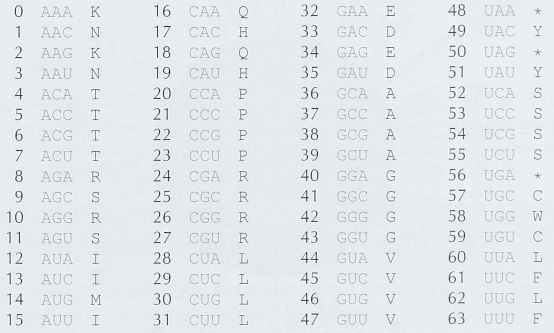
\includegraphics[width=0.8\textwidth]{poglavlja/4/slike/genetskiKod.png}
	\caption{Genetski kod.}
	\label{slika:genetskiKod}
\end{figure} 


Vidimo da se, na primer, kodon $UGG$ preslikava u aminokiselinu $Trp (W)$, dok se više kodona, $CUA, CUC, CUG, CUU, UUA, UUG$, preslikava u jednu aminokiselinu $Lys (L)$. 

Redom, kodone iz RNK preslikavamo u aminokiseline. Ali, kako znamo da je kraj nekog proteina? U genetskom kodu je i tako nešto kodirano. Postoje tzv. \textbf{stop kodoni} koji označavaju da iza njih nema više aminokiselina koje čine taj protein. Ti stop kodoni su $UAA, UAG, UGA$. 

\newpage


Dolazimo do jednog veoma značajnog biološkog aksioma -- \textbf{centralne dogme molekularne biologije}. Ona govori da se transkripcijom na osnovu DNK može dobiti RNK, a translacijom se iz RNK, na osnovu genetskog koda, dobijaju proteini. Ovu teoriju je predstavio Fransis Krik (eng. \textit{Francis Crick}) i prikazana je na slici \ref{slika:centralnaDogma}.
\begin{figure}[h!]
	\centering
	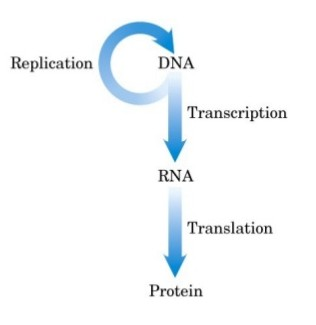
\includegraphics[width=0.5\textwidth]{poglavlja/4/slike/centralnaDog.jpg}
	\caption{Centralna dogma molekularne biologije.}
	\label{slika:centralnaDogma}
\end{figure} 



Ono što želimo da saznamo jeste koje aminokiseline i kojim redom ulaze u sastav našeg malog peptida tirocidina B1. Pošto se on sastoji iz 10 aminokiselina, to znači da ga čine 30 nukleotida u genomu bakterije \textit{Bacillus Brevis} koje će da se prepišu u RNK i da se prevedu iz RNK u tirocidin B1. Hiljade različitih $30$-grama se može prevesti u tirocidin B1 jer se u genetskom kodu različiti kodoni mogu prevesti u istu aminokiselinu. Na slici \ref{slika:30grami} su prikazani neki od takvih $30$-grama. Vidimo da oni nisu previše slični.
\begin{figure}[h!]
	\centering
	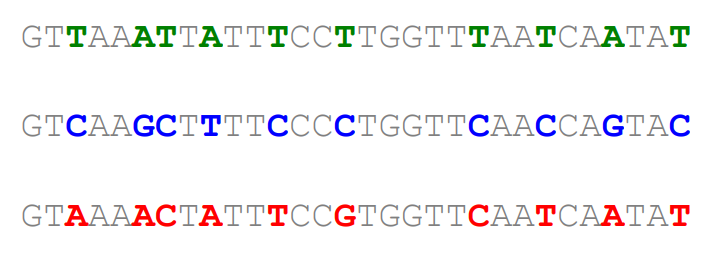
\includegraphics[width=0.8\textwidth]{poglavlja/4/slike/30grami.png}
	\caption{Neki od $30$-grama koji se mogu prevesti u tirocidin B1.}
	\label{slika:30grami}
\end{figure} 
\noindent

 Treba uzeti u obzir da translacija može početi na bilo kojoj poziciji u genomu. To znači da bismo za datu poziciju, ako gledamo $30$-gram, mogli da imamo 6 različitih tzv. \textbf{čitajućih okvira}, tj. 6 varijanti prepisivanja u RNK i onda prevođenja. Tri čitajuća okvira potiču iz tri nukleotida iz jednog kodona iz jednog prevedenog RNK lanca (ako krenemo da čitamo od prvog nukleotida, to je jedan čitajući okvir, iz drugog nukleotida je drugi čitajući okvir, iz trećeg nukleotida je treći čitajući okvir, a ako pročitamo od četvrtog nukleotida, to je već isti čitajući okvir kao prvi jer tu kreće novi kodon), a isto tako za drugi RNK lanac imamo tri čitajuća okvira sa druge strane. 

Naš peptid tirocidin B1 jeste \textit{cikličan}. Tih 10 aminokiselina koje ga čine idu nekim redom, ali su one povezane u krug, tako da imamo ukupno 10 različitih \textbf{linearnih reprezentacija} za tirocidin B1 u zavisnosti od toga koja nam je prva aminokiselina bila u samom receptu DNK. Koju god linearnu reprezentaciju pronađemo, rešili smo problem. 
\\\\
\indent Ne odustajemo od pronalaženja $30$-grama u genomu bakterije \textit{Bacillus Brevis} koji kodira bar jednu linearnu reprezentaciju od svih 10 koje čine tirocidin B1. Pretpostavimo da imamo na raspolaganju veoma moćan računar i neograničeno vreme. Doći ćemo do jednog čudnog rezultata. Nećemo uspeti da pronađemo nijedan $30$-gram u genomu bakterije \textit{Bacillus Brevis} koji kodira bar jednu linearnu reprezentaciju proteina tirocidina B1. Zašto? Stvari se komplikuju. Na ovom primeru je pokazano da centralna dogma ne važi uvek, odnosno ne važi da svaki protein u ćeliji nastaje na osnovu recepta koji je zapisan u DNK. Centralna dogma govori da se proces transkripcije izvršava pod uticajem enzima koji se zove \textit{RNK polimeraza}, a translacija RNK u protein se vrši u ćelijskoj organeli koja se naziva \textit{ribozom}. Postoje neki proteini koji ne nastaju na ovaj način, nego na specijalan način gde obično sekvenciranje genoma ne može da nam pomogne. Moramo da predložimo novi metod kako možemo da pronađemo odgovarajuću sekvencu aminokiselina. 

Edvard Tejtum (eng. \textit{Edward Tatum}), jedan od poznatih američkih genetičara, je 1963. godine inhibirao ribozom bakterije \textit{Bacillus Brevis}. Šta ovo znači? S obzirom da se znalo da se u ribozomu vrši translacija RNK u protein, on je onemogućio da se bilo šta desi u ribozomu, isključio je funkcionisanje te organele u ćeliji i očekivao je da se neće stvoriti nijedan protein, pa ni tirocidin B1. Međutim, suprotno očekivanjima, nastavljena je proizvodnja nekih peptida, uključujući i tirocidine. Ovo je bilo izuzetno iznenađujuće otkriće.

Fric Lipman (eng. \textit{Fritz Lipmann}), američko-nemački biohemičar, je 1969. godine  pokazao da tirocidini spadaju u grupu \textbf{ne-ribozomalnih peptida (NRP-ova)}. To su peptidi za čiju sintezu nisu odgovorni ribozomi i RNK polimeraza već enzimi poznati pod nazivom \textbf{NRP sintetaze}, molekuli koji se takođe nalaze u ćeliji i utiču na različite procese koji se dešavaju u njoj. To znači da se stvaranje tirocidina razlikuje od većeg broja proteina u živim bićima. 
\\\\
\indent Kako izgleda sinteza tirocidina B1 pomoću NRP sintetaze? Postoji veliki broj različitih NRP sintetaza, nije samo jedna odgovorna za stvaranje svih mogućih NRP-ova, nego za svaki ne-ribozomalni peptid postoji odgovarajuća NRP sintetaza. Ona NRP sintetaza koja je odgovorna za stvaranje tirocidina B1 se sastoji od 10 različitih podjedinica koje nazivamo \textit{moduli}. Svaki modul je odgovoran za nadovezivanje jedne aminokiseline na budući molekul tirocidina B1. Svaki od modula privuče jednu aminokiselinu i spoji je sa prethodnom, a poslednji korak jeste cirkularizacija -- spajanje aminokiselina nastalih uz pomoć prvog i poslednjeg modula radi kreiranja cikličnog peptida.

\section{Sekvenciranje antibiotika razbijanjem na komade} \label{razbijanje}

Pošto nam sekvenciranje genomske sekvence i pronalaženje odgovarajuće podniske koja je zadužena za translaciju u aminokiseline odgovarajućeg peptida ne može pomoći u sekvenciranju tirocidina B1 (jer on ne nastaje na osnovu informacije zapisane u DNK), postavljamo pitanje da li postoji način na koji možemo da sekvenciramo antibiotike. Moramo direktno da sekvenciramo peptid. Jedan od načina jeste \textbf{sekvenciranje razbijanjem na komade} i biće predstavljen u ovoj sekciji.
\\\\

\indent U sekvenciranju antibiotika može nam pomoći mašina koja se naziva \textbf{maseni spektrometar} i koju možemo opisati kao skupu molekularnu vagu. Šta on radi? Za početak ćemo da se zapitamo kako možemo da merimo težinu, tačnije masu molekula. 

Pošto se molekuli sastoje od atoma, prvo treba da govorimo o masi pojedinačnog atoma. U atomima postoje protoni, neutroni i elektroni. Protoni i neutroni su približno iste mase, dok su elektroni izuzetno mali i gotovo zanemarljive mase. Zato masu jednog atoma možemo svesti na masu protona, odnosno neutrona koji učestvuju u izgradnji konkretnog atoma koji posmatramo, pa se i masa molekula može izračunati kao suma masa atoma koji ga čine. Maseni spektrometar vraća masu molekula izračunatu u \textbf{Daltonima}. 
\begin{center}
$1 \quad Dalton (Da) \approx masa \quad jednog \quad protona/neutrona$ \\
$Masa \quad molekula \approx suma \quad masa \quad protona/neutrona$
\end{center}

Posmatrajmo masu jedne aminokiseline, recimo glicina. Glicin ima hemijsku formulu $ C_{2}H_{3}ON $. Ugljenik ima masu 12, vodonik ima masu 1, kiseonik 16, a azot 14. Na osnovu ovih masa računamo masu celog molekula glicina.
\begin{center}
$  masa(C_{2}H_{3}ON) = 12*2 + 1*3 + 16*1 + 14*1 \approx 57 Da $
\end{center}

\noindent Simbol  $ \approx $ koristimo jer nam je stvarna masa nešto malo drugačija od celobrojne mase koju dobijamo ovde. Stvarna masa glicina iznosi $ 57.02 Da $. Podrazumevaćemo da je masa celog molekula upravo celobrojna masa koju smo dobili.

Tabela masa svih aminokiselina data je u tabeli \ref{tabela:mase}.

\begin{center}
\begin{table} [h!]
\centering
\caption{Tabela masa 20 aminokiselina poređanih rastuće prema celobrojnim masama.}
\label{tabela:mase}
\begin{tabular}{ |c|c|c|c|c|c|c|c|c|c|c|c|c|c|c|c|c|c|c|c| } 
 \hline
 G & A & S & P & V & T & C & I,L & N &  D & K,Q & E & M & H & F & R & Y & W\\ 
 \hline 
 57 & 71 & 87 & 97 & 99 & 101 & 103 & 113 & 114 & 115 & 128 & 129 & 131 & 137 & 147 & 156 & 163 & 186 \\ 
 \hline
\end{tabular}
\end{table}
\end{center}

Primećujemo da neke aminokiseline imaju iste mase, npr. $I$ i $L$, $K$ i $Q$, pa za 20 aminokiselina imamo 18 celobrojnih masa.

Kada imamo mase aminokiselina, možemo da se zapitamo koja je masa tirocidina B1. Znajući da se tirocidin B1 sastoji iz 10 aminokiselina ovim redom: $ VKLFPWFNQY $, masu računamo koristeći tabelu \ref{tabela:mase}. 

\begin{center}
$  masa(tirocidina \quad B1) = 99+128+113+147+97+186+147+114+128+163 = 1322 $
\end{center}

Vratimo se na maseni spektrometar o kojem smo govorili ranije. Zamislimo da imamo kratak peptid koji se sastoji od samo 4 aminokiseline $NQEL$. Uzorak ovog peptida ubacimo u maseni spektrometar. Šta se u njemu dešava? U njemu se nekim hemijskim procesima, u čije detalje nećemo ulaziti, generišu svi podpeptidi ulaznog peptida. Sa računarske tačke gledišta, maseni spektrometar generiše od zadate niske $NQEL$ sve moguće podniske, podrazumevajući da je ulazni peptid cikličan. Tako se generišu podniske dužine jedan: $N, Q, E, L$, podniske dužine dva: $NQ, QE, EL, LN$ i podniske dužine tri: $NQE$, $QEL$, $ELN$, $LNQ$. Maseni spektrometar za svaki od dobijenih podpeptida može da odredi molekulsku masu. Ono što mi dobijemo kao izlaz iz masenog spektrometra nisu podpeptidi, mi ne znamo koje podpeptide je dobio, niti kojim podpeptidima je prudružena koja masa. Izlaz iz masenog spektrometra jeste samo niz masa! Taj izlazni niz može da sadrži i dva ista broja jer neki podpeptidi mogu da imaju istu masu.

Kako bismo formulisali računarski problem, moramo da definišemo šta je to \textit{teorijski spektar}. 
\begin{definicija} \textbf{Teorijski spektar peptida} predstavlja niz masa svih mogućih podpeptida tog peptida, uključujući nulu kao masu praznog peptida i masu samog peptida.
\end{definicija}

Poznajući sastav peptida, lako možemo da izračunamo teorijski spektar. Suprotan smer je težak, odnosno teško je da na osnovu teorijskog spektra zaključimo kako je izgledao peptid. Upravo ovo jeste problem sekvenciranja ciklopeptida.

\begin{problem}[Problem sekvenciranja ciklopeptida] 
	Rekonstruisati ciklični peptid na osnovu njegovog teorijskog spektra. \\
\end{problem}



\subsection{Sekvenciranje ciklopeptida grubom silom}

Kada dobijemo spektar iz masenog spektrometra, najveća masa će označavati masu celog peptida. Želimo prvo da generišemo sve peptide sa masom jednakom masi celog peptida, zatim da za svaki tako generisan peptid formiramo teorijski spektar i uporedimo ga sa datim spektrom. Algoritam grube sile za problem sekvenciranje ciklopeptida dat je u nastavku. 

\begin{lstlisting}
BFCyclopeptideSequencing(Spectrum)
begin
	// ParentMass(Spectrum) jeste najveca masa u spektru Spectrum
	for every Peptide with Mass(Peptide) equal to ParentMass(Spectrum)
		if Spectrum == CycloSpectrum(Peptide)
			output Peptide
end
\end{lstlisting}

Vidimo da u ovom algoritmu ispitujemo sve kandidate (peptide sa istom masom kao dati peptid). Koliko imamo takvih kandidata? Grafik koji oslikava odgovor na ovo pitanje dat je na slici \ref{slika:kolikoPeptida}.

\begin{figure}[h!]
	\centering
	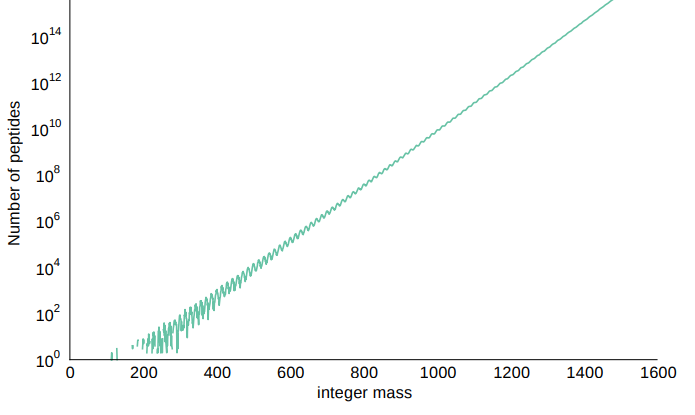
\includegraphics[width=0.7\textwidth]{poglavlja/4/slike/kolikoPeptida.png}
	\caption{Broj peptida sa zadatom masom.}
	\label{slika:kolikoPeptida}
\end{figure} 


Vidimo da je ovaj algoritam grube sile eksponencijalne složenosti. Pod uslovom da imamo dovoljno brz računar, ovako nešto bismo i mogli da izračunamo. Ali, šta bi bili nedostaci ovog algoritma grube sile? Možemo da imamo dva peptida sa istom masom, a da su potpuno različiti. Na primer, peptid $NQEL$ i peptid $TMDH$ imaju masu 484. Kako možemo da isključimo pogrešan peptid? Za oba ova peptida možemo da generišemo teorijski spektar. Ispostavlja se da su njihovi spektri potpuno različiti. Želimo da ovu informaciju iskoristimo u sledećem pristupu rešavanja problema sekvenciranja ciklopeptida. Cilj nam je da ne idemo grubom silom već da ogroman broj kandidata od samog početka odstranimo.
\newpage

\subsection{\textit{Branch-and-Bound} algoritam za sekvenciranje ciklopeptida}

U ovom pristupu postepeno konstruišemo kandidate za rešenja od manjih linearnih peptida za razliku od prethodnog pristupa u kome smo odmah generisali ceo peptid koji postaje kandidat. Na taj način ćemo smanjiti ukupan broj linearnih peptida koje posmatramo. Ovakav pristup se koristi kod \textbf{\textit{Branch-and-Bound} algoritama} koji će biti opisani u nastavku.

Kod \textit{Branch-and-Bound} algoritama u celokupnom prostoru svih mogućih rešenja vršimo nekakva odsecanja. Počnemo od kratkog peptida dužine jedan, pa ga proširimo na sve moguće načine, odnosno, dodamo po jednu aminokiselinu i od toga napravimo sve moguće kandidate dužine dva. To je \textit{branch grana} i predstavljena je na slici \ref{slika:branch}. \textit{Bound grana} bi od postojećih kandidata, nastalih u \textit{branch} granama, isključila neke potencijalne kandidate. \textit{Bound} grana je predstavljena na slici \ref{slika:bound}. Postupak proširivanja i odsecanja ponavljamo sve dok ne dođemo do odgovarajućih vrednosti. Na ovaj način će nam ostati mnogo manje kandidata za rešenja nego u prethodnom pristupu grube sile.

\begin{minipage}{\textwidth}
	\centering
	\begin{minipage}{0.45\textwidth}
		\begin{figure}[H]
			\centering
			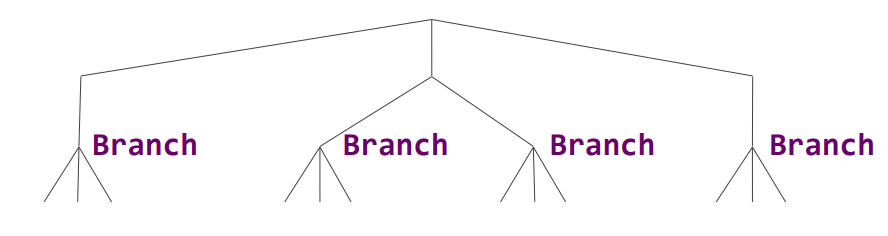
\includegraphics[width=\textwidth]{poglavlja/4/slike/branch.png}
			\caption{\textit{Branch} grane algoritma \textit{Branch-and-Bound}.}
			\label{slika:branch}
		\end{figure} 
	\end{minipage}
	\hfill 
	\begin{minipage}{0.45\textwidth}
		\begin{figure}[H]
			\centering
			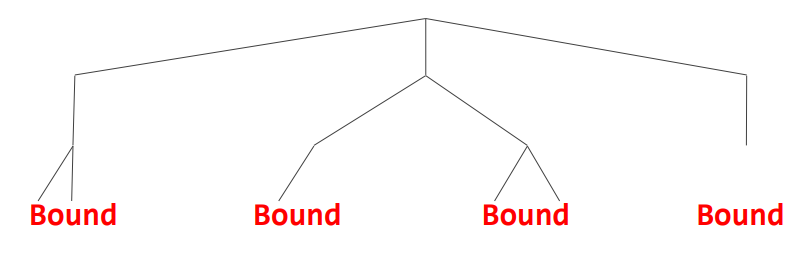
\includegraphics[width=\textwidth]{poglavlja/4/slike/bound.png}
			\caption{\textit{Bound} grane algoritma \textit{Branch-and-Bound}.}
			\label{slika:bound}
		\end{figure} 
	\end{minipage}
	\vspace*{1em}
\end{minipage}

Primenimo ovaj algoritam na konkretan problem. Recimo da nam je dat spektar
\begin{center}
 0 97 97 99 101 103 196 198 198 200 202 295 297 299 299 301 394 396 398 400 400 497.
 \end{center} 
\noindent  Vidimo da se u datom spektru nalaze mase nekih aminokiselina, što nam govori koje aminokiseline ulaze u sastav traženog peptida. Te aminokiseline su $P,V,T,C$ sa masama $97,99, 101, 103$. Ovo znači da možemo da počnemo ne sa svih 20 aminokiselina, nego sa 4 unigrama $P,V,T,C$. Ovo je unapred jedna \textit{bound} grana jer smo 20 aminokiselina sveli na 4 kandidata aminokiselina. Zatim idemo na branch granu, širimo unigrame u sve moguće bigrame: $PA$, $PC$, $PD$,..$PY$, $VA$, $VC$, $VD$,...,$VY$, $TA$, $TC$, $TD$,..., $TY$, $CA$, $CC$, $CD$,..., $CY$. Proširujemo sa svih 20 aminokiselina jer ćemo kasniji videti da ovako zadati spektar jeste čisto teorijski spektar, a maseni spektrometar skoro nikada u praksi ne vraća teorijski spektar već spektar sa nekakvim greškama. Kako možemo da skratimo ovu listu, kako možemo da izvršimo korak \textit{bound} u ovom trenutku? Posmatramo da li postoje odgovarajući bigrami koji se takođe pojavljuju u spektru. Zbog toga uvodimo pojam \textbf{konzistentnosti}.

\begin{definicija}
Za proizvoljan podpeptid $p_{1},..,p_{n}$ kažemo da je \textbf{konzistentan} sa spektrom $S$ ukoliko se svaka masa iz teorijskog spektra podpeptida  $p_{1},..,p_{n}$ nalazi u spektru $S$.
\end{definicija}

Na primer, $PV$ je \textbf{konzistentno} sa spektrom ukoliko se masa od $P$, masa od $V$ i masa od $PV$ nalaze u spektru.

Konzistentnost ćemo koristiti u \textit{bound} koraku, tačnije, izbacićemo sve bigrame koji nisu konzistentni sa spektrom. Tako dobijemo listu konzistentnih bigrama $PV$, $PT$, $PC$, $VP$, $VT$, $VC$, $TP$, $TV$, $CP$, $CV$ koju proširujemo u sve moguće $3$-grame, a zatim svodimo na listu samo konzistentnih $3$-grama. Postupak ponavljamo. Kada dođemo do liste konzistentnih pentagrama $PVCPT$, $PTPVC$, $PTPVC$, $PCVPT$, $VPTPC$, $VCPTP$, $TPVCP$, $TPCVP$, $CPTPV$, $CVPTP$ vidimo da zapravo svi oni pokazuju na jedan isti ciklični peptid.

Pseudokod opisanog algoritma dat je u nastavku.
\begin{lstlisting}
CyclopeptideSequencing(Spectrum)
begin
	Peptides = a set containing only the empty peptide
	while Peptides is non-empty
		// prosirujemo sve peptide u skupu sa svim mogucim aminokiselinama
		Peptides = Expand(Peptides)
		for each Peptide in Peptides
			// ParentMass(Spectrum) jeste najveca masa u spektru
			if Mass(Peptide) = ParentMass(Spectrum)
				if Cyclospectrum(Peptide) = Spectrum
					output Peptide
				remove Peptide from Peptides
			else if Peptide is not consistent with Spectrum
				remove Peptide from Peptides
end
\end{lstlisting}

Podsetimo se da je složenost algoritma grube sile, koji ovde pokušavamo da poboljšamo, eksponencijalna. Ispostavlja se da \textit{Branch-and-Bound} algoritam takođe može biti eksponencijalne složenosti za neke peptide, ali je u praksi veoma brz.



\section{Prilagođavanje sekvenciranja za spektre sa greškama} \label{greskeSpektri}

Spektar koji smo do sada definisali jeste teorijski spektar. Za razliku od njega, spektar koji izlazi iz masenog spektrometra, \textbf{eksperimentalni spektar}, često sadrže greške. O kakvim greškama se govori biće prikazano pomoću slike \ref{slika:ekspSpektar}.

\begin{figure}[h!]
	\centering
	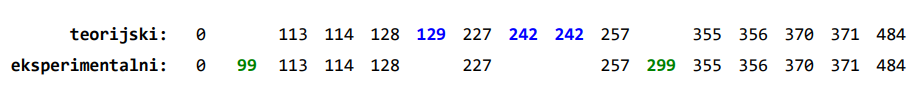
\includegraphics[width=0.9\textwidth]{poglavlja/4/slike/ekspSpektar.png}
	\caption{Primer teorijskog i eksperimentalnog spektra za $NQEL$.}
	\label{slika:ekspSpektar}
\end{figure} 

\textbf{Lažne mase} jesu mase koje su na slici \ref{slika:ekspSpektar} prikazane zelenom bojom. To su mase koje su prisutne u eksperimentalnom spektru, ali nisu prisutne u teorijskom spektru.

\textbf{Nedostajuće mase} jesu mase koje su na slici \ref{slika:ekspSpektar} prikazane plavom bojom. To su mase koje se nalaze u okviru teorijskog spektra, ali ne i u okviru eksperimentalnog spektra.

Zbog pojave ovih otežavajućih okolnosti, tj. grešaka u spektru, neophodan je novi algoritam jer se kod dva predložena algoritma teorijski spektar peptida morao u potpunosti poklapati sa spektrom peptida koji je predstavljao rešenje problema. Sada moramo da olabavimo taj uslov pa uvodimo pojam \textbf{skor peptida}.

\begin{definicija}
\textbf{Skor peptida} pokazuje koliko masa njegov teorijski spektar deli sa eksperimentalnim spektrom.
\end{definicija}

\noindent Tako, za sliku \ref{slika:ekspSpektar}, skor iznosi 11. Želimo da skor bude što veći.

S obzirom da imamo nov način upoređivanja, moramo da unapredimo naš \textit{Branch-and-Bound} algoritam, konkretno korak odsecanja. 

Uzmimo primer golfa. U golfu, kada igrači prođu prvi krug takmičenja, u sledeći krug prolaze dalje samo igrači koji su konkurentni, oni koji imaju šanse da nešto osvoje. To znači da možemo da kažemo da nam je odsecanje takvo da, na primer, prva tri igrača sa najboljim skorom idu dalje, a ukoliko imamo još neke igrače koji imaju isti skor kao poslednji igrač, onda i oni prolaze dalje. Znači, zadržavaju se tri najbolja igrača \textit{,,with ties''}. Ovakav sistem primenjen na \textit{Branch-and-Bound} algoritam prikazan je u sledećem pseudokodu.

\begin{lstlisting}
LeaderboardCyclopeptideSequencing(Spectrum, N)
begin
	Leaderboard = set containing only the empty peptide
	LeaderPeptide = empty peptide
	
	while Leaderboard is non-empty
		// prosirujemo sve elemente koji se nalaze u okviru skupa Leaderboard
		Leaderboard = Expand(Leaderboard)
		for each Peptide in Leaderboard
			// ParentMass(Spectrum) predstavlja najvecu masu u spektru Spectrum
			if Mass(Peptide) == ParentMass(Spectrum)
				if Score(Peptide, Spectrum) > Score(LeaderPeptide, Spectrum)
					LeaderPeptide = Peptide
			else if Mass(Peptide) > ParentMass(Spectrum)
				remove Peptide from Leaderboard
		// odsecamo kandidate iz Leaderboard na osnovu njihovog skora
		Leaderboard = Trim(Leaderboard, Spectrum, N)
		
	output LeaderPeptide
end

Trim(Leaderboard, Spectrum, N, AminoAcid, AminoAcidMass)
begin
	for j=1 to |Leaderboard|
		Peptide = j-th peptide in Leaderboard
		// LinearScore jeste skor nad linearnim spektrom
		LinearScores[j] = LinearScore(Peptide, Spectrum)
		
	sort Leaderboard according to the dec order of scores in LinearScores
	sort LinearScores in dec order
	
	for j=N+1 to |Leaderboard|
		if LinearScores[j] < LinearScores[N]
			remove all peptides starting from the j-th peptide from Leaderboard
			return Leaderboard
			
	return Leaderboard
end
\end{lstlisting}

\noindent \textit{Leaderboard} pristup omogućava da bolje definišemo za esperimentalni spektar kod \textit{Branch-and-Bound} algoritma onu bound fazu kada treba da izbacimo neke kandidate. 

\subsection{Testiranje na spektru tirocidina B1}

U ovom delu razmatraćemo rezultate testiranja na $Spectrum_{10}$, spektru sa 10\% lažnih/nedostajućih masa. 

Kada primenimo \textit{LeaderboardCyclopeptideSequencing} na spektar sa 10\% loših vrednosti, tada zaista dobijemo peptid sa najvišim skorom $ VKLFPWFNQY $  koji odgovara tirocidinu B1. Međutim, ukoliko uzmemo spektar $Spectrum_{25}$ koji ima 25\% lažnih i nedostajućih vrednosti, spektar koji se još više udaljava od teorijskog spektra, onda se peptid sa najvišim skorom $ VKLFPADFNQY $ razlikuje od peptida  $ VKLFPWFNQY $ koji želimo da dobijemo.

Ovo znači da \textit{LeaderboardCyclopeptideSequencing} algoritam radi dobro kada nam je eksperimentalni spektar malo različit od teorijskog.

\section{Od 20 do više od 100 aminokiselina} \label{viseAmino}

U ovoj sekciji biće reči o poboljšanju našeg algoritma uz uvođenje premisa koje postoje u stvarnosti, a koje smo do sada zanemarivali da bismo dali neke početne načine za rešavanje.

Kada smo govorili o proteinima, rekli smo da 20 aminokiselina najčešće učestvuje u njihovoj izgradnji i da su za nas, sa računarske tačke gledišta, proteini niske nad azbukom od 20 karaktera i da postoji još veliki broj aminokiselina nezavisno od izgradnje proteina u ćelijama živih bića. U gentskom kodu postoje kodovi samo za tih 20 aminokiselina, i u tabeli celobrojnih masa aminokiselina postoje mase samo za iste te aminokiseline. S obzirom da u ovom poglavlju razmatramo NRP peptide, peptide koji ne nastaju prema pravilima centralne dogme,  onda ovi peptidi mogu da sadrže i neke nestandardne aminokiseline, one aminokiseline koje se ne nalaze među standardnih 20 aminokiselina. Na primer, tirocidin B sadrži nestandardnu aminokiselinu \textit{Ornitin (Orn)}. Za Ornitin ne postoji nukleotidni triplet u okviru genetskog koda na osnovu koga se ova aminokiselina dobija i ne postoji celobrojna masa u tabeli celobrojnih masa za aminokiseline. S ozbirom na to, možemo da pretpostavimo da bilo koji ceo broj između 57 i 200 (koliko nam iznosi najmanja i najveća masa standardnih aminokiselina) može biti masa neke nestandardne aminokiseline. Ovako nešto može da izgleda kao grubo ograničenje, ali je eksperimentalno potvrđeno da većina masa svih mogućih aminokiselina pripada ovom intervalu.

Spektar u kome nismo ograničeni na tabelu od samo 18 celobrojnih masa, već uzimamo u obzir da bilo koji celi broj između 57 i 200 može da označava neku aminokiselinu, nazivamo \textbf{prošireni spektar}. Kada primenimo Leaderboard algoritam na prošireni spektar sa 10\% lažnih i nedostajućih masa, peptid koji dobijemo $  VKLFPWFN-98-65 $ sadrži neke vrednosti za mase koje ne odgovaraju nijednoj aminokiselini. Pošto Leaderboard algoritam ovde ne daje ispravne vrednosti, moramo da primenimo jedan sasvim novi princip.

\section{Spektralna konvolucija} \label{konvolucija}

Kod algoritma sa proširenim spektrom podrazumeva se da svi celi brojevi između 57 i 200 odgovaraju masama aminokiselina. To znači da razmatramo 144 ili više (znamo da jednoj masi može da odgovara više aminokiselina, a sa druge strane postoje vrednosti kojima ne odgovara nijedna) aminokiselina u koje spadaju i standardne i nestandardne aminokiseline. Želimo da smanjimo broj aminokiselina koje razmatramo. 

Posmatrajmo eksperimentalni spektar za $ NQEL $
\begin{center}
0 99 113 114 128 227 257 299 355 356 370 371 484.
\end{center}
\noindent Mi znamo da je $ Mass(E) = 129 $ i vidimo da u spektru ne postoji ta vrednost. Sa druge strane, u spektru postoji $ Mass(QE) = 257 $ i $ Mass(Q) = 128 $. Razlika ove dve mase daje vrednost $129$. Ova vrednost već deluje kao dobra vrednost za nedostajuću masu. U spektru postoji još ovakvih slučajeva. Recimo, $ Mass(ELN) - Mass(LN) = 356 - 227 = 129 $ i $ Mass(NQEL) - Mass(LNQ) = 484 - 355 = 129 $. Obe ove razlike ukazuju na masu od $E$ koja nedostaje.

Uvodimo tabelu koja se naziva \textbf{spektralna konvolucija}.
\begin{definicija}
\textbf{Spektralna konvolucija} je tabela koja pokazuje apsolutnu vrednost razlike između svake dve mase u spektru.
\end{definicija}

Primer spektralne konvolucije za spektar čije su lažne vrednosti označene sa ,,false'' prikazan je na slici \ref{slika:spektralnaKonvolucija}.

\begin{figure}[h!]
	\centering
	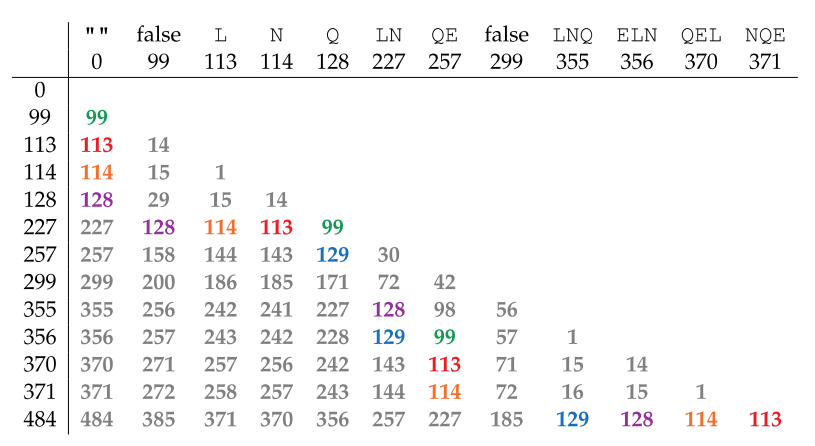
\includegraphics[width=0.9\textwidth]{poglavlja/4/slike/spektralnaKonvolucija.png}
	\caption{Primer spektralne konvolucije.}
	\label{slika:spektralnaKonvolucija}
\end{figure}

\noindent Na preseku svake vrste i kolone u spektralnoj konvoluciji upisana je apsolutna vrednost razlike celobrojnih masa. Kako iskoristiti spektralnu konvoluciju? Tražimo vrednosti razlika koje se pojavljuju najveći broj puta, a da se nalaze između 57 i 200. Obojene vrednosti na slici \ref{slika:spektralnaKonvolucija} se pojavljuju veći broj puta. To su vrednosti 99, 113, 114, 128 i 129. Ove vrednosti odgovaraju masama aminokiselina, redom, $V, L, N, Q, E $. Od 5 najčešćih aminokiselina u konvoluciji 4 čine peptid $NQEL$.

Kako bi izgledao unapređeni algoritam za sekvenciranje ciklopeptida ukoliko uzmemo u obzir i nestandardne aminokiseline, odnosno proširenu tabelu celobrojnih masa aminokiselina? Pseudokod je dat u nastavku.
\begin{lstlisting}
ConvolutionCyclopeptideSequencing(Spectrum, N, M)
begin
	Formirati spektralnu konvoluciju spektra Spectrum.
	Uzeti M najcescih elemenata u konvoluciji (izmedju 57 i 200).
	Primeniti LeaderboardCyclopeptideSequencing, formirajuci peptide samo na osnovu ovih M celih brojeva.
end
\end{lstlisting}

Algoritam  \textit{ConvolutionCyclopeptideSequencing} daje tačan rezultat i za spektre sa šumom od 10\% i za spektre sa šumom od 25\%, što pokazuje da je spektralna konvolucija odgovorila na sve izazove koji su postavljeni.

\section{Spektri u realnosti} \label{realnost}

Kao što znamo, realnost je obično drugačija. Neke poteškoće iz realnosti smo zanemarivali. Koje?
\begin{itemize}
	\item $Spectrum_{25}$ je mnogo manje šumovit nego spektri dobijeni u praksi iz masenog spektrometra.
	
	\item Maseni spektrometar ne meri jednostavno fragmente podpeptida, već su postupci merenja mnogo komplikovaniji. Najpre se zaista vrši razbijanje datog peptida na fragmente. Zatim se oni sortiraju, korišćenjem elektromagnetnog polja, prema svojoj masi. Ono što maseni spektrometar meri jeste zapravo \textbf{odnos mase i naelektrisanja} za svaki fragment (znači nije baš masa) i određuje \textbf{intenzitet} (kao broj jona) u svakom odnosu mase i naelektrisanja. Šta to znači? To znači da kao izlaz iz masenog spektrometra ne dobijamo eksperimentalni spektar koji smo do sada imali prilike da vidimo, nego grafik intenziteta prema odnosu mase i naelektrisanja sa vrhovima na određenim mestima. Primer ovakvog grafika dat je na slici \ref{slika:intenzitet}.
	\begin{figure}[h!]
	\centering
	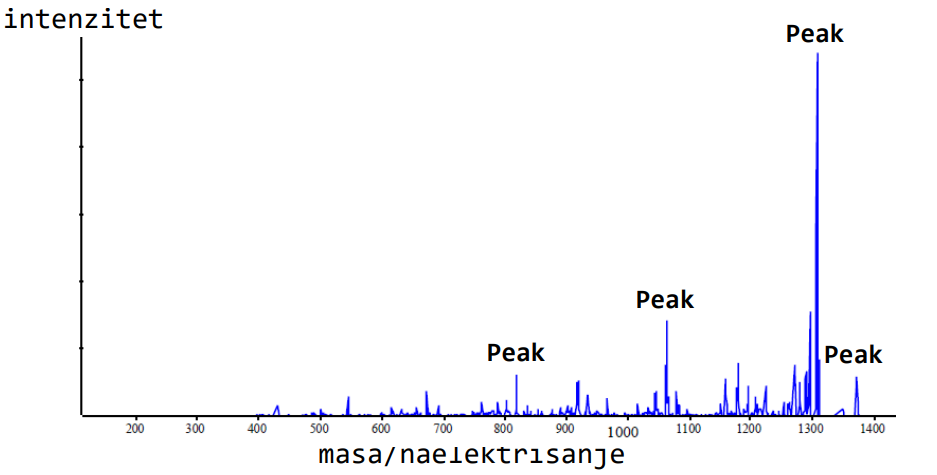
\includegraphics[width=0.9\textwidth]{poglavlja/4/slike/intenzitet.png}
	\caption{Primer grafika intenziteta prema odnosu mase i naelektrisanja.}
	\label{slika:intenzitet}
\end{figure}
	Na osnovu vrhova na grafiku, određivaćemo sam sastav peptida. Ovaj grafik se naziva \textbf{realni spektar}. Rekonstrukcija peptida na osnovu realnog spektra biće obrađena u poglavlju 11.
	
\end{itemize}

\newpage
\section{Zadaci sa vežbi}
\setexamplecodestyle

U nastavku će biti predstavljeni zadaci sa vežbi na kursu rađeni u programskom jeziku Python.

\subsection{Linear Spectrum}

\lstinputlisting[language=Python]{poglavlja/4/kodovi/LinearSpectrum.py}

\subsection{Cyclic Spectrum}

\lstinputlisting[language=Python]{poglavlja/4/kodovi/CyclicSpectrum.py}

\subsection{Cyclopeptide Sequencing}

\lstinputlisting[language=Python]{poglavlja/4/kodovi/CyclopeptideSequencing.py}

\subsection{Leaderboard Cyclopeptide Sequencing}

\lstinputlisting[language=Python]{poglavlja/4/kodovi/LeaderboardCyclopeptideSequencing.py}
\chapter{Kako poredimo biološke sekvence?}
\setbookcodestyle

\section{Biološki uvid u poređenje sekvenci}

Kako su biološke sekvence podložne promeni, umetanju i brisanju, čest je slučaj da i-ti simbol jedne sekvence odgovara simbolu na drugoj poziciji druge sekvence. U tom slučaju, cilj je postići najbolje poklapanje simbola.
Na primer, $ATGCATGC$ i $TGCATGCA$ nemaju delove koji se poklapaju, pa je njihova Hamingova udaljenost 8:

\begin{center}
$ATGCATGC$\\
$TGCATGCA$
\end{center}
    
Ali ako ih malo drugačije poravnamo, ove dve niske imaju 6 poklapajucih pozicija:

\begin{center}
$A\textcolor{red}{TGCATGC}-$\\
$-\textcolor{red}{TGCATGC}A$
\end{center}

Stringovi ATGCTTA i TGCATTAA imaju manje uocljive slicnosti:

\begin{center}
$A\textcolor{red}{TGC}-\textcolor{red}{TTA}-$\\
$-\textcolor{red}{TGC}A\textcolor{red}{TTA}A$
\end{center}

Ovi primeri navode nas da definisemo dobro poravnanje kao ono koje ima najveći mogući broj poklapanja. Povećanje broja poklapanja simbola možemo posmatrati kao igricu u kojoj u svakom potezu imamo dva izbora. Možemo da uklonimo oba simbola i osvojimo poen ako su oni isti ili mozemo ukloniti simbol iz jedne od niski, ne osvojimo poene, ali omogućimo da u daljem igranju osvojimo više poena. Cilj je da maksimizujemo broj poena.


%%%%%%%%%%%%%%%%%%%%%%%% ALEX
\section{Igra poravnanja i najduža zajednička podsekvenca}

Kod \textbf{Igre poravnanja} cilj je ukloniti sve simbole iz
sekvenci tako da pritom sakupimo što više poena :
\begin{itemize}
    \item Uklanjanje prvog simbola iz svake sekvence
            \item \textcolor{red}{1} poen ako se simboli poklapaju,  \textcolor{purple}{0} ako se simboli ne poklapaju
    \item Uklanjanje prvog simbola iz jedne sekvnce
         \begin{itemize}
            \item 0 poena
        \end{itemize}
\end{itemize}

\begin{figure}[h!]
\centering
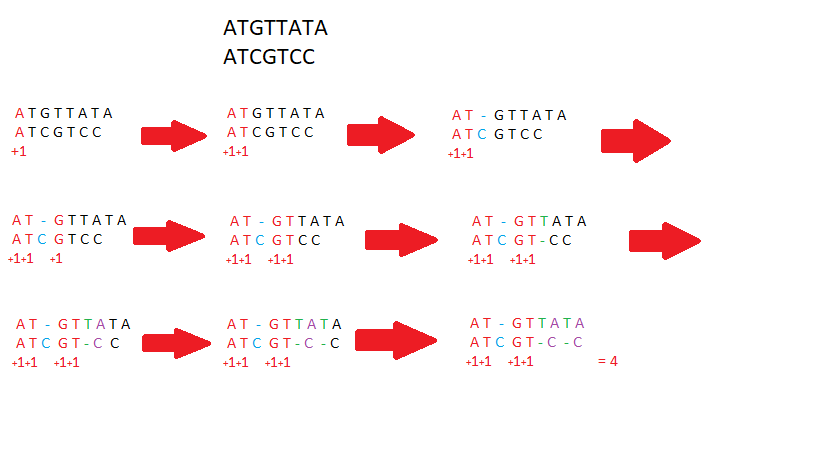
\includegraphics[width=0.7\textwidth]{poglavlja/5/slike/igraPoravnavanja.png}
\caption{Igra poravnanja}
\end{figure} 

\textbf{Poravnanje} dve sekvence predstavlja matricu koja ima dva reda:

\begin{enumerate}
    \item red: simboli prve sekvence (redom) eventualno sa ubačenim “-” 
    \item red: simboli druge sekvence (redom) eventualno sa ubačenim “-” 
\end{enumerate}
\begin{figure}[h!]
\centering
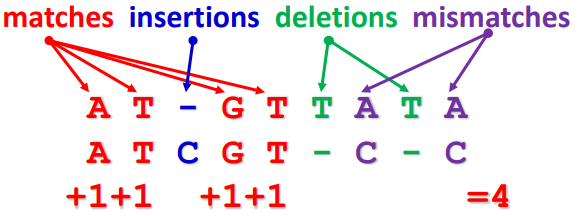
\includegraphics[width=0.4\textwidth]{poglavlja/5/slike/poravnanje.png}
\caption{Poravnanje}
\label{slika:poravnavanje}
\end{figure} 

\subsection{Najduža zajednička podsekvenca}

Poklapanja (matches) u poravnanju dve sekvence ( u primeru \ref{slika:poravnavanje} to je ATGT) formiraju njihovu zajedničku podsekvencu.
\begin{problem}[Problem najduže zajedničke podniske]
	Naći najdužu zajedničku podsekvencu dve niske. \\
	Ulaz: Dve niske. \\
	Izlaz: Najduža zajednička podsekvenca ovih niski
\end{problem}
%%%%%%%%%%%%%%%%%%%%%%%%%%%%%%%%%%%%%%%%%%%%

\section{Problem turiste na Menhetnu}

\noindent Pre svega postavimo problem:\\

\begin{problem}[Problem turiste na Menhetnu]
	Naći najdužu putanju u pravougaonoj mreži gradskih ulica. \\
	Ulaz: Usmeren težinski mrežni graf. \\
	Izlaz: Najduža putanja od početnog (source) do krajnjeg čvora (sink) u mrežnom grafu. 
\end{problem}

\begin{figure}[h!]
\centering
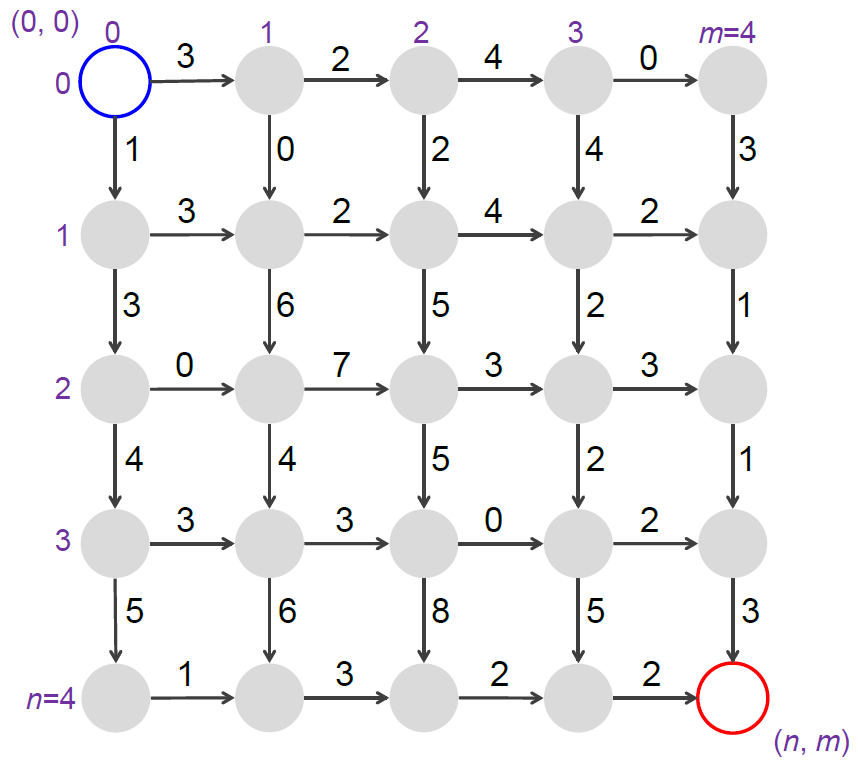
\includegraphics[width=0.7\textwidth]{poglavlja/5/slike/menhetn2.png}
\caption{Problem turiste na Menhetnu}
\label{slika:menhetn}
\end{figure} 

Na slici \ref{slika:menhetn} grafički je prikazan problem turiste na Menhetnu. Cilj je stići od plavog do crvenog kruga i pri tom sakupiti što više poena. Dozvoljeno kretanje je dole i desno. Možemo koristiti pohlepni algoritam i tako doći do cilja, ali da li smo tako sakupili najviše poena?

\noindent Dodatna izmena grafa bi bila da imamo i dijagnalne grane (\ref{slika:menhetn3}).

\begin{figure}[h!]
\centering
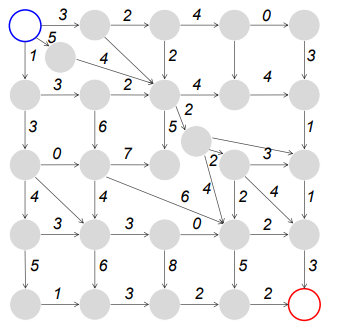
\includegraphics[width=0.7\textwidth]{poglavlja/5/slike/menhetn3.png}
\caption{Nepravilna mreža}
\label{slika:menhetn3}
\end{figure}

\noindent Time dolazimo do sledećeg problema:

\begin{problem}[Problem najduže putanje u usmerenom grafu]
	Naći najdužu putanju između dva   čvora u težinskom usmerenom grafu. \\
	Ulaz: Usmereni težinski graf sa označenim
čvorovima source i sink. \\
	Izlaz: Najduža putanja od čvora source do čvora
sink u usmerenom težinskom grafu. 
\end{problem}

Ako se prisetimo igre poravnanja, videćemo da postoji veza između ova dva problema (igre).

\begin{figure}[h!]
\centering
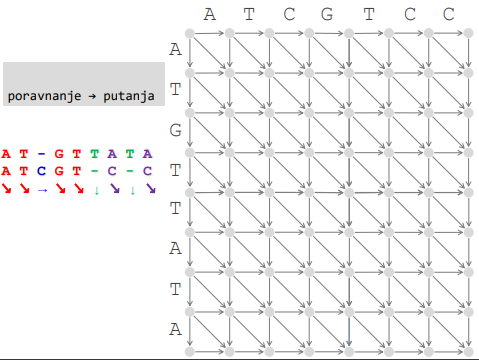
\includegraphics[width=0.7\textwidth]{poglavlja/5/slike/menhetn4.png}
\caption{Poravnanje $\rightarrow$ Putanja}
\label{slika:menhetn4}
\end{figure}

Pitamo se kako izgraditi graf za igru poravnanja i za problem najduže podsekvence. To ćemo uraditi na sledeći način:

\begin{itemize}
    \item Vrste označimo aminokiselinama iz prve niske
    \item Kolone označimo aminokiselinama iz druge niske
    \item U svaku presečnu tačku postavimo jedan čvor
    \item Gde god je moguće, postaviti vertikalne (insercija), horizontalne (delecija) i dijagonalne grane (match ili mismatch)
    \item Dijagonalne grane otežati koeficijentom 1, ostale koeficijentom 0
    \item Problem najduže zajedničke podsekvence se svodi na problem nalaženja najduže putanje između dva data čvora u usmerenom grafu
\end{itemize}

Kada nađemo poravnanje najvišeg skora našli smo i najdužu putanju u mrežnom grafu.

\begin{figure}[h!]
\centering
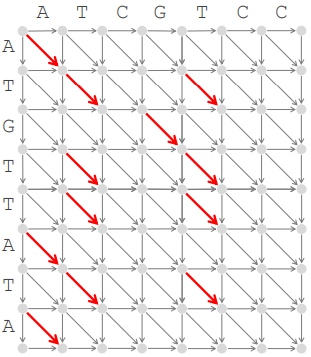
\includegraphics[width=0.7\textwidth]{poglavlja/5/slike/poravnanje1.png}
\caption{Poravnanje $\rightarrow$ Putanja}
\label{slika:poravnanje2}
\end{figure}

Dijagonalne crvene grane odgovaraju poklapanju simbola i imaju skor 1 (\ref{slika:poravnanje2})

%%%%%%%%%%%%%%%%%%%%%%%%%%%%%%%%%%%%%jasmina%%%%%%%%%%%%%%%%%%%%%%%%%%%%%%%%%%%%%%%%%%%%%%%%%%%%%%%%%%%%%%%%%%%%%%%%%%%%%%%%%%%%%%%%%%%%%%%%%%%%%%%%
\section{Problem kusura}

\noindent Upoznajmo se sa sledećim problemom:\\

\begin{problem}[Problem vraćanja kusura]
	Naći minimalan broj novčića neophodnih za vraćanje kusura. \\
	Ulaz: Ceo broj money i niz pozitivnih celih brojeva $(coin_1, coin_2, ..., coin_d)$. \\
	Izlaz: Minimalan broj novčića $(coin_1, coin_2, ..., coin_d)$ u apoenima koji rasitnjava sumu money. \\
\end{problem}

\subsection{Pohlepni algoritam}

Najzastupljeniji način vraćanja kusura širom sveta podrazumeva iterativno traženje sledećeg najvećeg novčića.\\
To bi značilo da bismo za kusur od 42 dinara dobili sledeće novčiće: 20 + 10 + 10 + 2. \\
Ovakav način vraćanja kusura opisuje takozvani pohlepni algoritam. \\

\begin{lstlisting}
GreedyChange(money)
begin
    change %$\leftarrow$% empty collection of coins
	while money > 0
		coin %$\leftarrow$% largest denomination that does not exceed money
		add coin to change
		money %$\leftarrow$% money - coin
	return change
end
\end{lstlisting}

Međutim, ako malo bolje razmislimo ovo rešenje zapravo nije najbolje.\\
Kusur bismo mogli vratiti i sa manje novčića na sledeći način: 42 = 20 + 20 + 2 \\

\textit{Zaključak}: \textbf{GreedyChange ne daje optimalno rešenje!}

\subsection{Rekurzivni algoritam}

Pokušajmo sada da problem rešimo na drugačiji način koristeći rekurziju. \\
Za zadate apoene 6, 5, 1, koji je najmanji broj novčića neophodnih za vraćanje kusura od 9 centi? \\

\begin{figure}[h!]
\centering
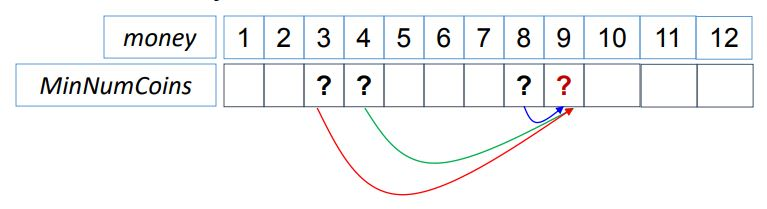
\includegraphics[width=0.7\textwidth]{poglavlja/5/slike/rekurzija1.JPG}
\caption{Vracanje kusura - rekurzija}
\label{slika:rekurzija}
\end{figure}

Problem resavamo tako sto prvo od 9 oduzmemo 6 i dobijemo 3 kao ostatak kusura. Dakle, 9 se može vratiti od jednog novčića od 6 apoena i jos plus broj novčiča koji je potreban za preostali deo kusura od 3 centa. \\
U istoj iteraciji analogno računamo za preostale apoene.\\

Na slici \ref{slika:rekurzija} crvenim znakom pitanja označeno je traženo rešenje koje dobijemo rešavanjem manjih problema za kusure 3, 4 i 8. \\ 

MinNumCoins(9) = $\min$ 
$\begin{cases}$
$MinNumCoins(9-6) + 1 = MinNumCoins(3) + 1\\$
$MinNumCoins(9-5) + 1 = MinNumCoins(4) + 1\\$
$MinNumCoins(9-1) + 1 = MinNumCoins(8) + 1\\$
$\end{cases}$

Na osnovu prethodnog, moguće je izvesti opštu formulu:

MinNumCoins(money) = $\min$ 
$\begin{cases}$
$MinNumCoins(money-coin_{1}) + 1 \\$
$\dots \\$
$MinNumCoins(money-coin_{d}) + 1 \\$
$\end{cases}$
\\
Hajde sada da vidimo kako bismo to isprogramirali:
\\
\begin{lstlisting}
RecursiveChange(money, coins)
begin
    if money = 0
        return 0
    MinNumCoins %$\leftarrow$% infinity 
    for i %$\leftarrow$% 1 to |coins|
        if money %$\geq coin_{i}$%
            NumCoins %$\leftarrow$% RecursiveChange(money - %$coin_{i}$%, coins)
            if numCoins + 1 < MinNumCoins
                MinNumCoins %$\leftarrow$% numCoins + 1
	return MinNumCoins
end
\end{lstlisting}

Reklo bi se da smo sada dobili odgovarajuci algoritam za naš problem, hajde to da proverimo. \\
Postavlja se pitanje, koliko je brz RecursiveChange? \\

Pokušajmo na konkretnom primeru da dođemo do rešenja. Neka naš problem sada bude vraćanje kusura od 76 centi. Pomoću rekurzivnog stabla demonstrirajmo ponašanje našeg algoritma: \\

\begin{figure}[h!]
\centering
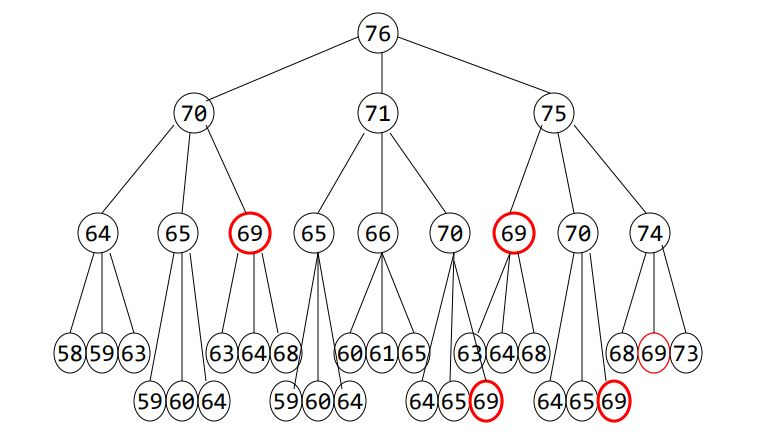
\includegraphics[width=0.7\textwidth]{poglavlja/5/slike/rekurzivnoStablo.JPG}
\caption{Vracanje kusura - ponašanje rekurzivnog algoritma}
\label{slika:rekurzija2}
\end{figure}

Ono što se odmah može primetiti jeste višestruko pozivanje algoritma za vrednost od 69 centi, čak 6 puta! \\
Daljim procenama možemo doći do zaključka da se optimalna kombinacija novčića za 30 centi izračunava milijardama puta! \\

Sada je očigledno da nam rekurzija ne rešava problem na najbolji mogući način. \\

\subsection{Vraćanje kusura dinamičkim programiranjem}

Cilj nam je da izbegnemo višestruka izračunavanja  vraćanja kusura za istu vrednost, tako da bi ideja bila da imamo objekat koji će pamtiti sva računanja i iz koga ćemo čitati već izračunate vrednosti. \\
Dakle, umesto vremenski zahtevnih poziva \\
\begin{center}
RecursiveChange(money - $coin_{i}$, coins)
\end{center}
jednostavno bismo potražili vrednosti iz unapred izračunate tabele \\
\begin{center}
MinNumCoins(money - $coin_{i}$).
\end{center}


\begin{lstlisting}
DPChange(money, coins)
begin
    MinNumCoins(0) %$\leftarrow$% 0 
    for m %$\leftarrow$% 1 to money
        MinNumCoins(m) %$\leftarrow$% infinity
        for i %$\leftarrow$% 1 to |coins|
            if m %$\geq coin_{i}$%
                if MinNumCoins(m - %$coin_{i}$%) + 1 < MinNumCoins(m)
                    MinNumCoins(m) %$\leftarrow$% MinNumCoins(m - %$coin_{i}$%) + 1
	return MinNumCoins(money)
end
\end{lstlisting}


\section{Dinamičko programiranje i putokazi za povratak}

Posmatramo jednostavniji, Menhetn graf:
Pretpostavimo da do čvora sink možemo doći samo na dva načina: kretanjem južno $\downarrow$ ili kretanjem istočno $\rightarrow$

\begin{figure}[h!]
\centering
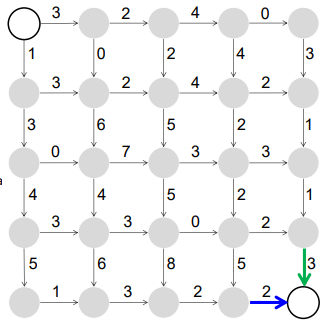
\includegraphics[width=0.7\textwidth]{poglavlja/5/slike/putokazi.png}
\caption{Južno ili istočno?}
\label{slika:putokazi}
\end{figure}

\noindent Prvo probamo da rešimo problem rekurzivno:

\begin{lstlisting}
SouthOrEast(n, m)
if n=0 and m=0
    return 0
x %$\leftarrow$% -infinity, y %$\leftarrow$% -infinity
if n > 0
x %$\leftarrow$% SouthOrEast(n-1,m)+weight of edge "%$\downarrow$%" into (n, m)
if m > 0
y %$\leftarrow$% SouthOrEast(n,m-1)+ weight of edge "%$\rightarrow$%" into (n,m)
return max{x, y}
\end{lstlisting}

\noindent Ovaj algoritam se poziva za svaki čvor u grafu veličine $m\times n$, a pri tom se dešava da za jedan isti čvor računamo više puta. Zbog toga je ovaj pristup previše spor, pa prelazimo na dinamičko programiranje.
Krenućemo  od početnog čvora. Zatim, u čvor (i, j) upisujemo dužinu maksimalne putanje od (0,0) do (i,j). Prvo izračunamo za čvorove na obodu grafa a zatim, kolonu po kolonu, za preostale čvorove.

\begin{figure}[h!]
\centering
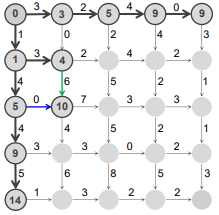
\includegraphics[width=0.5\textwidth]{poglavlja/5/slike/putokazi1.png}
\caption{Južno ili istočno?}
\label{slika:putokazi1}
\end{figure}

\begin{figure}[h!]
\centering
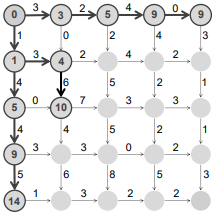
\includegraphics[width=0.5\textwidth]{poglavlja/5/slike/putokazi2.png}
\caption{Južno ili istočno?}
\label{slika:putokazi2}
\end{figure}

\begin{figure}[h!]
\centering
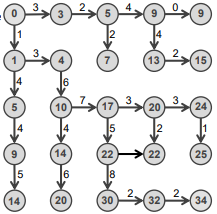
\includegraphics[width=0.5\textwidth]{poglavlja/5/slike/putokazi3.png}
\caption{Južno ili istočno?}
\label{slika:putokazi3}
\end{figure}

Na slici \ref{slika:putokazi3} prikazane su podebljane grane koje predstavljaju putokaze za povratak od čvora sink do čvora source.

\subsection{Rekurentna relacija dinamičkog programiranja kod Menhetn grafa}

$s_i,_j$: the length of a longest path from (0,0) to (i,j)

$s_i,_j$ = $\max$ $\begin{cases}$
$s_{i-1},_j + weight of edge "\downarrow"into (i,j)\\$
$s_i,_{j-1} + weight of edge "\rightarrow"into (i,j)$
$\end{cases}$

\begin{lstlisting}
ManhattanTourist(n, m, Down, Right)
%$s_0,_0$% %$\leftarrow$% 0
for i %$\leftarrow$% 1 to n
    %$s_i,_0$% %$\leftarrow$% %$s_{i-1},_0$% + %$down_i,_0$%
for j %$\leftarrow$% 1 to m
    %$s_0,_j$% %$\leftarrow$% %$s_0,_{j-1}$% + %$right_0,_j$% 
for i %$\leftarrow$% 1 to n
    for j %$\leftarrow$% 1 to m
        %$s_i,_j$% %$\leftarrow$% %$\max$% { %$s_{i-1},_j$% + %$down_i,_j$%, %$s_i,_{j-1}$% + %$right_i,_j$% }
return %$s_n,_m$%
\end{lstlisting}



%%%%%%%%%%%%%%%%%%%%%%%%%%%%%%%%%%%%%%%%%%%%%%%%%%%%%%%%%%%%%%%%%%%%%%%%%

\section{Od Menhetna do grafa poravnanja }

\subsection{Rekurentna relacija dinamičkog programiranja kod grafa poravnanja}


Najduži put (slika \ref{slika:povratak}) od (0,0) do (i,j) se računa:


$s_i,_j$ = $\max$ $\begin{cases}$
$s_{i-1},_j$ + 
$\textcolor{green}{weight\ of\ edge\ "\downarrow"\ into\ (i,j)}\\$
$s_i,_{j-1}$ + 
$\textcolor{blue}{weight\ of\ edge\ "\rightarrow"\ into\ (i,j)}\\$
$s_{i-1},_{j-1}$ + 
$\textcolor{red}{weight\ of\ edge\ "\searrow"\ into\ (i,j)}$
$\end{cases}$

Što dalje daje :

$s_i,_j$ = $\max$ $\begin{cases}$
$\textcolor{green}{s_{i-1},_j + 0}\\$
$\textcolor{blue}{s_i,_{j-1} + 0}\\$
$\textcolor{red}{s_{i-1},_{j-1} + 1, v_i = w_j}\\$
$\textcolor{red}{s_{i-1},_{j-1} + 0, v_i \neq w_j}$
$\end{cases}$



\begin{figure}[h!]
\centering
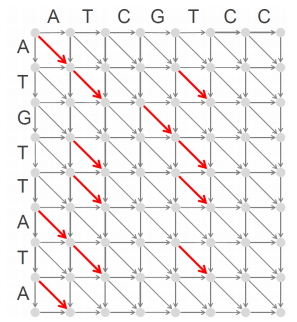
\includegraphics[width=0.5\textwidth]{poglavlja/5/slike/graf1.png}
\caption{ Crvene grane težina 1, ostale grane težina 0, $v_i$ i $w_j$ oznake vrste i kolone}
\label{slika:povratak}
\end{figure}


U slici \ref{slika:backtrack} se vide boldovane grane koje su nastale primenom pravila rekurentne relacije. One predstavljaju putokaze za povratak (backtrack) kod grafa za najdužu zajedničku podsekvencu. 

\begin{figure}[h!]
\centering
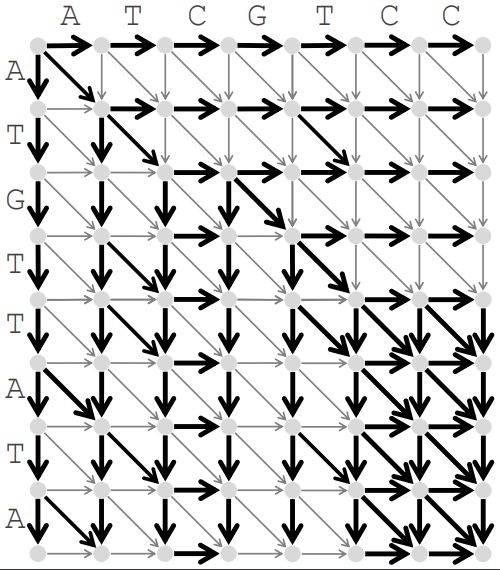
\includegraphics[width=0.5\textwidth]{poglavlja/5/slike/backtrack.png}
\caption{Putokazi za povratak (backtrack)}
\label{slika:backtrack}
\end{figure}

\subsection{Računanje putokaza za povratak }

$s_i,_j$ $\leftarrow$ $\max$ $\begin{cases}$
$\textcolor{green}{s_{i-1},_j + 0}\\$
$\textcolor{blue}{s_i,_{j-1} + 0}\\$
$\textcolor{red}{s_{i-1},_{j-1} + 1, v_i = w_j}\\$
$\textcolor{red}{s_{i-1},_{j-1} + 0, v_i \neq w_j}$
$\end{cases}$


$backtrack_i,_j$  $\leftarrow$  $\max$ $\begin{cases}$
$\textcolor{blue}{ "\rightarrow", s_i,_j = s_{i},_{j-1}}\\$
$\textcolor{green}{ "\downarrow", s_i,_j = s_{i-1},_j}\\$
$\textcolor{red}{"\searrow", otherwise}$
$\end{cases}$


Podsetimo se sada kako bismo rekontruisali putanju preko putokaza kod Menhetn grafa? Krenuli bismo od krajnjeg čvora (sink) i pratili putokaze u obrnutom smeru do početnog čvora (source) \ref{slika:rek3}.\\
\begin{figure}[h!]
\centering
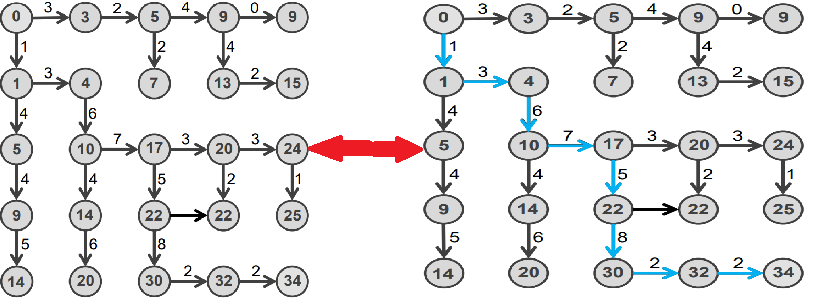
\includegraphics[width=0.7\textwidth]{poglavlja/5/slike/rek3.png}
\caption{Rekonstrukcija putanje preko putokaza kod Menhetn grafa}
\label{slika:rek3}
\end{figure}

\begin{figure}[h!]
\centering
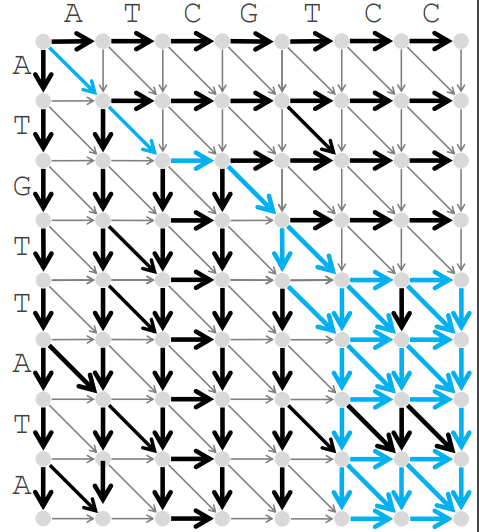
\includegraphics[width=0.5\textwidth]{poglavlja/5/slike/backtrackNajduzaZajPS.png}
\caption{Backtracking}
\label{slika:backNZPS}
\end{figure}
Sada na slici \ref{slika:backNZPS} možemo videti povratak (backtracking) kod grafa za najdužu zajedničku podsekvencu.

\subsection{Određivanje najduže zajedničke podsekvence (LCS – longest common subsequence) korišćenjem putokaza za povratak}

\begin{lstlisting}
OutputLCS (backtrack, v, i, j)
if i = 0 or j = 0
    return
if %$backtrack_i,_j$% = "%$\rightarrow$%"
    OutputLCS (backtrack, v, i, j-1)
else if %$backtrack_i,_j$% = "%$\downarrow$%"
    OutputLCS (backtrack, v, i-1, j)
else
    OutputLCS (backtrack, v, i-1, j-1)
    output  %$v_i$%
\end{lstlisting}

Do sada smo pretpostavljali da graf u kom tražimo
najdužu putanju ima samo tri vrste grana. Da li se OutputLCS može generalizovati tako da važi i za grafove koji nemaju tako specifičnu
topologiju?\\
Kako se rekurentna relacija dinamičkog programiranja menja za ovakav graf? \ref{slika:rekRel}
\begin{figure}[h]
\centering
\includegraphics[width=\textwidth]{poglavlja/5/slike/rekurentaRelDinProg.png}
\caption{}
\label{slika:rekRel}
\end{figure}
\\

\textit{$s_a$ = $max_{all\ predecessors\ b\ of\ node\ a}$\{$s_b$+ weight of edge from b to a\}}
\\

Računanje skora za SVE prethodnike \ref{slika:racunanje}.

\begin{figure}[h]
\centering
\includegraphics[width=0.7\textwidth]{poglavlja/5/slike/racunanje.png}
\caption{Začarani krug}
\label{slika:racunanje}
\end{figure}

\begin{itemize}
    \item Kod ovakve rekurentne relacije, važno je da pri računanju $s_a$ imamo izračunate $s_b$ za sve čvorove prethodnike b (čvorovi za koje
postoji grana do čvora a) Da li je to moguće u bilo kom usmerenom
težinskom grafu? Odgovor je \textbf{nije}. Da bismo kod svakog čvora mogli da mogli da izračunamo skor za sve njegove prethodnike, usmereni težinski graf mora biti acikličan. DAG (Directed Acyclic Graph) 
    \item Ako je dat usmereni aciklični graf, da li njegove čvorove možemo poređati u niz tako da njihov redosled u nizu osigurava uslov da pri računanju $s_a$ imamo izračunate $s_b$ za sve čvorove prethodnike b (čvorovi za koje postoji grana do čvora a)? Odgovor je \textbf{da}, moguće je poređati sve čvorove grafa u niz i taj niz topološki sortirati
\end{itemize}




\subsection{Topološko sortiranje}

\begin{itemize}
    \item \textbf{Topološko sortiranje} : Sortiranje čvorova DAG-a u nizu tako da sve grane u takvom nizu idu s leva na desno.
    \item \textbf{ Teorema}: Svaki DAG se može topološki sortirati.
    \item Topološko sortiranje svakog DAG-a se obavlja za O(\#edges) koraka.
\end{itemize}

\textbf{Algoritam za nalaženje najduže putanje u DAG-u>} :

\begin{lstlisting}
LongestPath(Graph, source, sink)
for each node a in Graph
     %$s_a$% %$\leftarrow$% -%$\infty$%
%$s_{source}$% %$\leftarrow$%  0
topologically order Graph
for each node a (from source to sink in topological order)
%$s_a$%  %$\leftarrow$% %$max_{all\ predecessors\ b\ of\ node\ a}$% {%$s_b$% + weight of edge from b to a}
return %$s_{sink}$%
\end{lstlisting}


\begin{itemize}
    \item Pošto svaka grana učestvuje tačno jednom, složenost je O(\#edges)
    \item LongestPath vraća dužinu najdužeg zajedničkog podniza ali ne rekonstruiše putanju
\end{itemize}

%%%%%%%%%%%%%%%%%%%%%%%jasminaaaaaa%%%%%%%%%%%%%%%%%%%%%%%%%%%%%%%%%%%%%%%%%
\section{Od globalnog do lokalnog poravnanja}

\noindent Uvedimo sledeće:
\begin{itemize}
    \item Skor poravnanja do sada - $\#\textcolor{red}{matches}$ \\
    \item Skor sa mismatch i indel kaznama - $\#\textcolor{red}{matches} - \textcolor{purple}{\mu} * \#\textcolor{purple}{mismatches} - \sigma * \#\textcolor{blue}{in}\textcolor{green}{dels}$ \\
\end{itemize}

Primer na slici \ref{slika:matriceSkora}. \\

\begin{figure}[H]
\centering
\includegraphics[width=\textwidth]{poglavlja/5/slike/matriceSkora.JPG}
\caption{}
\label{slika:matriceSkora}
\end{figure}

Navedimo rekurentnu relaciju dinamičkog programiranja kod grafa poravnanja. Počinjemo od:

$s_i,_j$ = $\max$ $\begin{cases}$
$s_{i-1},_j$ + 
$\textcolor{green}{weight\ of\ edge\ "\downarrow"\ into\ (i,j)}\\$
$s_i,_{j-1}$ + 
$\textcolor{blue}{weight\ of\ edge\ "\rightarrow"\ into\ (i,j)}\\$
$s_{i-1},_{j-1}$ + 
$\textcolor{red}{weight\ of\ edge\ "\searrow"\ into\ (i,j)}$
$\end{cases}$

Odnosno, \\
\\
$s_i,_j$ = $\max$ $\begin{cases}$
$\textcolor{green}{s_{i-1},_j - \sigma}\\$
$\textcolor{blue}{s_i,_{j-1} - \sigma}\\$
$\textcolor{red}{s_{i-1},_{j-1} + 1, v_i = w_j}\\$
$\textcolor{purple}{s_{i-1},_{j-1} - \mu, v_i \neq w_j}\\$
$\end{cases}$
\\
A uz pomoc funkcije $score()$ može se zapisati i kao: \\
\\

\begin{figure}[!htb]
     \begin{minipage}{0.49\textwidth}
        $s_i,_j$ = $\max$ $\begin{cases}$
        $\textcolor{green}{s_{i-1},_j + score(v_i, -)}\\$
        $\textcolor{blue}{s_i,_{j-1} + score(-, w_j)}\\$
        $\textcolor{red}{s_{i-1},_{j-1} score(v_i, w_j)}\\$
        $\end{cases}$
     \end{minipage}
     \hfill
     \begin{minipage}{0.49\textwidth}
       \includegraphics[width=\linewidth]{poglavlja/5/slike/rekurentna.JPG}
       \caption{}\label{}
     \end{minipage}
   \end{figure}
   
\subsection{Globalno poravnanje}

\begin{problem}[Problem globalnog poravnanja]
	Naći poravnanje sa najvišim skorom između dve niske za datu matricu skora. \\
	Ulaz: Niske v i w, kao i matrica skora score \\
	Izlaz: Poravnanje niski v i w čiji je skor poravnanja (prema matrici skora) maksimalan od svih mogućih poravnanja v i w. 
\end{problem}

\noindent Šta bi bili homeobox geni? \\
\begin{itemize}
    \item Dva gena u različitim vrstama mogu biti slična u kratkim, konzervativnim regionima, a različita u ostalim delovima.
    \item Homeobox geni sadrže kratak region homeodomen koji je čvrsto konzerviran među različitim vrstama.
    \item Globalno poravnanje može da propusti nalaženje homeodomena jer pokušava da poravna sekvence u celosti.
\end{itemize}

\noindent Uporedimo sledeća dva poravnanja: \\
\begin{figure}[!htb]
 \begin{minipage}{0.49\textwidth}
    \includegraphics[width=\linewidth]{poglavlja/5/slike/globalno.JPG}
   \caption{}\label{}
   score = 22(matches) - 2(indent) = 2
 \end{minipage}
 \hfill
 \begin{minipage}{0.49\textwidth}
   \includegraphics[width=\linewidth]{poglavlja/5/slike/lokalno.JPG}
   \caption{}\label{}
   score = 17 (matches) - 30(indent) = -13
 \end{minipage}
\end{figure}
   
\begin{figure}[!htb]
 \begin{minipage}{0.49\textwidth}
    \includegraphics[width=\linewidth]{poglavlja/5/slike/grafik_poravnanje1.JPG}
   \caption{}\label{}
 \end{minipage}
 \hfill
 \begin{minipage}{0.49\textwidth}
   \includegraphics[width=\linewidth]{poglavlja/5/slike/grafik_poravnanje2.JPG}
   \caption{}\label{}
 \end{minipage}
\end{figure}

\noindent Ako se zapitamo koje od njih je bolje, iz priloženog zaključujemo da je to lokalno poravnanje.\\

\subsection{Lokalno poravnanje}

Lokalno poravnanje računamo kao globalno poravnanje u pravougaoniku, pogledajmo sliku \ref{slika:pravougaonici}. \\

\begin{figure}[H]
 \begin{minipage}{0.49\textwidth}
    \includegraphics[width=\linewidth]{poglavlja/5/slike/lokalno_poravnanje_pravougaonici1.JPG}
   \caption{}\label{}
 \end{minipage}
 \hfill
 \begin{minipage}{0.49\textwidth}
   \includegraphics[width=\linewidth]{poglavlja/5/slike/lokalno_poravnanje_pravougaonici2.JPG}
   \caption{}\label{slika:pravougaonici}
 \end{minipage}
\end{figure}

\noindent Da bismo dobili lokalno poravnanje potrebno je da izračunamo globalno poravnanje u okviru svakog pravougaonika.\\
Algoritam globalnog poravnanja ponovićemo između svaka dva čvora, ne samo između početnog (source) i krajnjeg (sink). \\
Stoga, broj ponavljanja algoritma će biti $\#nodes ^ 2$ puta. \\

\begin{problem}[Problem lokalnog poravnanja]
	Naći lokalno poravnanje najvećeg skora između dve niske. \\
	Ulaz: Niske v i w, kao i matrica skora score \\
	Izlaz: Podniske niski v i w čije je globalno poravnanje (prema matrici skora) maksimalno među svim globalnim poravnanjima svih podniski niski v i w. 
\end{problem}

\noindent Zamislimo da postoji taksi koji bi nas besplatno vozio do tačke početka lokalnog poravnanja, i od tačke završetka lokalnog poravnanja pa do kraja. Na taj način ne bismo skupili negativne poene, već samo pozitivne. Ovakva vožnja nam daje samo skor lokalnog poravnanja kao što smo i želeli. \ref{slika:taksiFree}\\
 
 \begin{figure}[H]
\centering
\includegraphics[width=0.7\textwidth]{poglavlja/5/slike/free_taxi.JPG}
\caption{Besplatne taksi vožnje}
\label{slika:taksiFree}
\end{figure} 

Konstruišimo Menhetn graf za problem lokalnog poravnanja: \\

\begin{figure}[H]
     \begin{minipage}{0.59\textwidth}
        Kako bi izgledao Menhetn graf za nas problem? \\
        Dodamo grane težine 0 od (0,0) do svakog čvora, i od svakog čvora do (n,m). \\
        Ukupan broj dodatih grana je $O(|v|+|w|)$, pa algoritam ostaje brz. \\
     \end{minipage}
     \hfill
     \begin{minipage}{0.39\textwidth}
       \includegraphics[width=\linewidth]{poglavlja/5/slike/free_taxi_graf.JPG}
       \caption{Menhetn graf za lokalno poravnanje}\label{}
    \end{minipage}
\end{figure}

Problem rešavamo dinamičkim programiranjem: \\

\begin{figure}[H]
     \begin{minipage}{0.59\textwidth}
        $s_i,_j$ = $\max$ $\begin{cases}$
        $s_{i-1},_j$ + 
        $\textcolor{green}{weight\ of\ edge\ "\downarrow"\ into\ (i,j)}\\$
        $s_i,_{j-1}$ + 
        $\textcolor{blue}{weight\ of\ edge\ "\rightarrow"\ into\ (i,j)}\\$
        $s_{i-1},_{j-1}$ + 
        $\textcolor{red}{weight\ of\ edge\ "\searrow"\ into\ (i,j)}$
        $\end{cases}$
     \end{minipage}
     \hfill
     \begin{minipage}{0.39\textwidth}
       \includegraphics[width=\linewidth]{poglavlja/5/slike/lokalno_poravnanje_0.JPG}
       \caption{weight of (0,0) into (i,j) = 0}\label{}
    \end{minipage}
\end{figure}


%%%%%%%%%%%%%%%%%%%%%%%%%%%%%%%%%%%%%%%%%%%%%%%%%%%%%%%%%%%%%%%%%%%%
\section{Kažnjavanje insercija i delecija u poravnanju sekvenci}

\subsection{Kažnjavanje praznina}

\begin{itemize}
    \item U globalnom poravnanju je fiksna kazna $\sigma$ bila dodeljena svakom indelu
    \item Međutim, ova fiksna kazna može biti preoštra
kod lokalnog poravnanja kada možemo imati 100 uzastopnih indela.
    \item Niz od k uzastopnih indela često predstavlja jedan isti evolucioni događaj, ne k različitih, slika \ref{slika:kaznjavanje}
\end{itemize}

\begin{figure}[h]
\centering
\includegraphics[width=0.5\textwidth]{poglavlja/5/slike/kaznjavanjePraznina.png}
\caption{}
\label{slika:kaznjavanje}
\end{figure}

\subsection{Adekvatnije kazne za praznine}

\textbf{Afina kazna za praznine} za prazninu dužine k:  \textbf{$\sigma+\epsilon*(k-1)$}
\begin{itemize}
    \item $\sigma$ kazna za \textbf{otvaranje} praznine
    \item $\epsilon$ kazna za \textbf{proširenje} praznine
    \item $ \sigma > \epsilon$ , jer otvaranje praznine treba kazniti više nego njeno proširenje
\end{itemize}



U slici \ref{slika:modelovanje} prikayano je modelovanje afinih kazni za praznine pomoću dugih grana.

\begin{figure}[h!]
\centering
\includegraphics[width=0.7\textwidth]{poglavlja/5/slike/modelovanjePomocuDugihGrana.png}
\caption{Modelovanje afinih kazni za praznine pomoću dugih grana}
\label{slika:modelovanje}
\end{figure}

\subsection{Izgradnja Menhetn grafa sa afinim kaznama za praznine}

\begin{figure}[h!]
\centering
\includegraphics[width=0.5\textwidth]{poglavlja/5/slike/MenhettnAifnePraznine.png}
\caption{Dodali smo $O(n^3)$ grana}
\label{slika:afiniMenhetn}
\end{figure}


\begin{itemize}
    \item Vremenska složenost je direktno proporcionalna broju grana, zbog čega želimo da smanjimo broj grana u grafu (trenutno je
$O(n^3)$ \ref{slika:afiniMenhetn})
\item Jedan način za smanjivanje broja grana je povećanje broja čvorova u grafu
\item Zato delimo Menhetn graf na tri nivoa \ref{slika:triNivoa}
\end{itemize}


\begin{figure}[h!]
\centering
\includegraphics[width=\textwidth]{poglavlja/5/slike/triNivoa.png}
\caption{Podela Menhetna grafa na 3 nivoa}
\label{slika:triNivoa}
\end{figure}

Ako imamo putanju poput one na slici \ref{slika:kakoSimulirati}, kako da je predstavimo pomoću Menhetn grafa na 3 nivoa? Rešenje je prikazano na slici \ref{slika:simulacija}


\begin{figure}[h!]
\centering
\includegraphics[width=0.5\textwidth]{poglavlja/5/slike/kakoSimulirari.png}
\caption{Kako predstaviti pomoću Menhetn grafa na 3 nivoa?}
\label{slika:kakoSimulirati}
\end{figure}


\begin{figure}[h!]
\centering
\includegraphics[width=0.7\textwidth]{poglavlja/5/slike/simulacija.png}
\caption{Simulacija Menhetn grafa na 3 nivoa}
\label{slika:simulacija}
\end{figure}

%%%%%%%%%%%%%%%%%%%%%%%%%%%%%%%%%jasminaaaa%%%%%%%%%%%%%%%%%%%%%%%%%%%%%%%%%%%

\section{Prostorno efikasno poravnanje sekvenci}

Zapitajmo se sledeće: \\
Da li možemo poravnati NPR sintetaze iz dve različite bakterije? \\
\\

Uzmimo u obzir sledeće činjenice:
\begin{itemize}
    \item NPR sintetaze su obično veoma dugi proteini, približno 20 000 aminokiselina
    \item Vremenska složenost poravnanja je probližno jednaka broju ivica (\#edges), odnosno kvadratna
    \item Prostorna složenost poravnanja je probližno jednaka broju čvorova (\#nodes), odnosno kvadratna
    \item \textbf{Memorija je često usko grlo pri poređenju dugih sekvenci}
\end{itemize}

Iz prethodnog zaključujemo da nam prostorna složensot pravi problem i da bi za prosečan racunar ovo bilo nemoguće da izračuna. 
Stoga, potreban nam je drugi pristup koji će nam rešiti problem. Potreban nam je algoritam koji zahteva linearnu prostornu složenost i udvostručenu vremensku složenost. U te svrhe najčešće se koristi algoritam koji radi po principu podeli-pa-vladaj. \\

Uvedimo nove pojmove:
\begin{itemize}
    \item Srednja kolona poravnanja (middle) $= \#columns/2$, slika \ref{slika:srednjaKolona}
    \item Srednji čvor poravnanja - čvor u preseku putanje optimalnog poravnanja i srednje kolone, slika \ref{slika:srednjiCvor}
\end{itemize}


\begin{figure}[h!]
\centering
\includegraphics[width=0.5\textwidth]{poglavlja/5/slike/srednjaKolona.JPG}
\caption{Srednja kolona poravnanja}
\label{slika:srednjaKolona}
\end{figure}

\begin{figure}[h!]
\centering
\includegraphics[width=0.5\textwidth]{poglavlja/5/slike/srednjiCvor.JPG}
\caption{Srednji čvor poravnanja}
\label{slika:srednjiCvor}
\end{figure}

Koristeći navedene pojmove, demonstrirajmo algoritam \textbf{Podeli-pa-vladaj} za poravnanje sekvenci, slika \ref{slika:podeliPaVladaj}: \\

\begin{lstlisting}
AlignmentPath(source, sink)
    find middleNode
    AlignmentPath(source, middleNode)
    AlignmentPath(middle, sink)
\end{lstlisting}

\begin{figure}[h!]
\centering
\includegraphics[width=0.5\textwidth]{poglavlja/5/slike/podeliPaVladaj.JPG}
\caption{Srednja kolona poravnanja}
\label{slika:podeliPaVladaj}
\end{figure}

\subsection{Prostorna složenost}
Za nalaženje najduže putanje u grafu poravnanja traži se čuvanje svih putokaza za - $O(nm)$ prostora. \\
Međutim, za nalaženje dužine najduže putanje u grafu poravnanja ne traži se čuvanje svih putokaza - $O(n)$ prostora, slika \ref{slika:prostornaSlozenost}

\begin{figure}[h!]
\centering
\includegraphics[width=0.5\textwidth]{poglavlja/5/slike/prostornaSlozenost2.JPG}
\caption{Recikliranje prostora za kolone u grafu poravnanja}
\label{slika:prostornaSlozenost}
\end{figure}

Dobijamo da je prostor potreban za algoritam $2*n \sim O(n)$, odnosno, linearan. \\ 

\subsection{Vremenska složenost}

Neka je \textbf{i-putanja} najduža putanja od svih putanja koja posećuje i-ti čvor u srednjoj koloni i neka je \textbf{$length(i)$} dužina i-putanje.\\

Na slici \ref{slika:iputanja} vidimo da je $length(0)=2$ i $length(4)=4$. \\


\begin{figure}[h!]
\centering
\includegraphics[width=0.5\textwidth]{poglavlja/5/slike/i_putanje.JPG}
\caption{Računanje length(i)}
\label{slika:iputanja}
\end{figure}


$length(i)$ možemo računati na sledeći način:
\begin{center}
$length(i) = fromSource(i) + toSink(i)$
\end{center}

\begin{figure}[h!]
\centering
\includegraphics[width=0.5\textwidth]{poglavlja/5/slike/i_putanje.JPG}
\caption{Računanje length(i)}
\label{slika:iputanja}
\end{figure}

Na slici \ref{slika:sourceSink} vidimo koliko je potrebno vremena za nalaženje srednjeg čvora - čak $O(nm)$ vremena za nalaženje samo jednog čvora! 
\begin{figure}[h!]
\centering
\includegraphics[width=0.5\textwidth]{poglavlja/5/slike/sourceSink.JPG}
\caption{Računanje vremena za nalaženje srednjeg čvora}
\label{slika:sourceSink}
\end{figure}

Svaki problem se može rešiti u vremenu proporcionalnom broju grana tj. površini koju zauzima. \\
Vreme potrebno za rešavanje naredna dva potproblema: $area/4 + area/4 = area/2$, znači  $O(nm + nm/2)$ vremena za nalaženje 3 čvora. \\
Dakle, vreme potrebno za nalaženje svih čvorova je: $area + area/2 + area/4 + area/8 + \dots < 2 * area$! Slika \ref{slika:vreme} vizuelno prikazuje vreme potrebno za nalaženje 7 tačaka. \\

\begin{figure}[h!]
\centering
\includegraphics[width=0.5\textwidth]{poglavlja/5/slike/vremenskaSlozenostPPV.JPG}
\caption{Računanje vremena za nalaženje 7 tačaka}
\label{slika:vreme}
\end{figure}

Pokazali smo da je vremenska složenost $2*n*m \sim O(n*m)$. \\
%%%%%%%%%%%%%%%%%%%%%%%%%%%%%%%%%%%%%%%%%%%%%%%%%%%%%%%%%%%%%%%%%%%%

\section{Višestruko poravnanje sekvenci}

\subsection{Od dvostrukog do višestrukog poravnanja}
\begin{itemize}
    \item Do sada su u poravnanju učestvovale samo dve sekvence.
    \item Slaba sličnost između dve sekvence postaje značajna ako je prisutna i u drugim sekvencama
    \item Višestruka poravnanja mogu otkriti suptilne sličnosti koje dvostruka poravnanja ignorišu
\end{itemize}

\subsection{Poravnanje tri A-domena}
Na slici \ref{slika:poravnavanjaTriA} je prikazano poravnanje tri A-domena
\begin{figure}[h!]
\centering
\includegraphics[width=\textwidth]{poglavlja/5/slike/poravnavanjaTriAdomena.png}
\caption{Poravnavanja 3 A-domena}
\label{slika:poravnavanjaTriA}
\end{figure}

\subsection{Generalizacija dvostrukog na višestroko poravnanje}
    
\begin{itemize}
    \item Poravnanje 2 sekvence je matrica od 2 reda
    \item Poravnanje 3 sekvence je matrica od 3 reda (slika  \ref{slika:poravnavanjeMatrica})
    \begin{figure}[h!]
    \centering
    \includegraphics[width=0.3\textwidth]{poglavlja/5/slike/poravnanjeMatrica.png}
    \caption{}
    \label{slika:poravnavanjeMatrica}
    \end{figure}
    \item Funkcija skora treba da dodeljuje visok skor poravnanjima sa konzerviranim kolonama
\end{itemize}



\subsection{Poravnanja = 3-D putanje}

Poravnanje sekvenci ATGC, AATC i ATGC \ref{slika:3d}

\begin{figure}[h]
\centering
\includegraphics[width=0.8\textwidth]{poglavlja/5/slike/3dPoravnanja.png}
\caption{Poravnanje sekvenci ATGC, AATC i ATGC}
\label{slika:3d}
\end{figure}

\subsection{2-D poravnanje u odnosu na 3-D poravnanje}
\begin{figure}[h]
\centering
\includegraphics[width=0.5\textwidth]{poglavlja/5/slike/2d3d.png}
\caption{}
\label{slika:2d3d}
\end{figure}
2-D poravnanje u odnosu na 3-D poravnanje prikazano na slici \ref{slika:2d3d}.

\subsection{Rekurentna relacija dinamičkog programiranja
za višestruko poravnanje}



$s_i,_j,_k$ = $\max$ $\begin{cases}$

$s_{i-1},_{j-1},_{k-1}$+ $\delta(v_i, w_j, u_k)\\$
$s_{i-1},_{j-1},_k$+ $\delta(v_i, w_j, -)\\$
$s_{i-1},_j,_{k-1}$+ $\delta(v_i, -, u_k)\\$
$s_i,_{j-1},_{k-1}$+ $\delta(-, w_j, u_k)\\$
$s_{i-1},_{j},_k$+ $\delta(v_i,-, -)\\$
$s_{i},_{j-1},_k$+ $\delta(-, w_j, -)\\$
$s_{i},_{j},_{k-1}$+ $\delta(-, -, u_k)\\$
$\end{cases}$

$\delta$(x, y, z) - element 3-D matrice skora

\subsection{Vremenska složenost dinamičkog algoritma
za višestruko poravnanje}

\begin{itemize}
    \item Kao kod dvostrukog poravnanja, vremenska složenost je proporcionalna broju grana O(\#edges)
    \item Za 3 sekvence n, vremenska složenost je proporcionalna 7$n^3$
    \item Za poravnanje k sekvenci, potrebno je izgraditi kdimenzionalni Menhetn graf sa: 
    \begin{itemize}
        \item  $n^k$ čvorova
        \item većina čvorova će imati $2^k – 1$ ulaznih grana
        \item Vremenska složenost: O($2^kn^k$)
    \end{itemize}
\end{itemize}


Višestruko poravnanje uključuje i dvostruko poravnanje, slika \ref{slika:visestrukoDvostruko}

\begin{figure}[h!]
\centering
\includegraphics[width=0.5\textwidth]{poglavlja/5/slike/visestrukoDvostruko.png}
\caption{}
\label{slika:visestrukoDvostruko}
\end{figure}

\subsection{Da li se višestruko poravnanje može izgraditi iz dvostrukog?}
Za dati skup proizvoljnih dvostrukih poravnanja, možemo li konstruisati višestruko poravnanje iz kog su izvedeni (slika \ref{slika:dvostruka})?

\begin{figure}[h!]
\centering
\includegraphics[width=0.7\textwidth]{poglavlja/5/slike/dvostruka.png}
\caption{}
\label{slika:dvostruka}
\end{figure}

\subsection{Profilna reprezentacija višestrukog poravnanja}

Na slici \ref{slika:profilVisetruko} prikazana profilna reprezentacija višestrukog poravnanja.
\begin{figure}[h!]
\centering
\includegraphics[width=0.6\textwidth]{poglavlja/5/slike/profilVisestruko.png}
\caption{}
\label{slika:profilVisetruko}
\end{figure}


\begin{itemize}
    \item Do sada smo poravnavali \textbf{sekvencu u odnosu na sekvencu.}
    \begin{itemize}
        \item Možemo li poravnati \textbf{sekvencu u odnosu na profil}?
        \item Možemo li poravnati \textbf{profil u odnosu na profil}?
    \end{itemize}
   
\end{itemize}


\subsection{Višestruko poravnanje: pohlepni pristup}

\begin{itemize}
    \item Izabrati najsličnije sekvence i kombinovati ih u profil
     \item Tako bismo smanjili broj sekvenci sa k na k-2 i jedan profil
    \item Iterirati
\end{itemize}

Primer pohlepnog pristupa:
\begin{itemize}
    \item Sekvence: GATTCA, GTCTGA, GATATT, GTCAGC
    \item 6 dvostrukih poravnanja (\textcolor{red}{match}+1, \textcolor{ForestGreen}{in}\textcolor{blue}{dels} i \textcolor{purple}{mismatches -1}) slika \ref{slika:sestDvostrukih}
    \begin{figure}[h!]
    \centering
    \includegraphics[width=0.5\textwidth]{poglavlja/5/slike/sestDvostrukih.png}
    \caption{}
    \label{slika:sestDvostrukih}
    \end{figure}
    \item Pošto su $s_2$ i $s_4$ najbliže, od njih pravimo profil
    
     \begin{figure}[h!]
    \centering
    \includegraphics[width=0.4\textwidth]{poglavlja/5/slike/profil.png}
    \caption{}
    \label{slika:profil}
    \end{figure}
    \item Novi skup od 3 sekvence za poravnanje:\\
            $s_1$ GATTCA\\
            $s_3$ GATATT\\
            $s_2,_4$ \textcolor{ForestGreen}{GTC}\textcolor{red}{t/a}\textcolor{ForestGreen}{G}\textcolor{red}{a/c}

\end{itemize}
%%% dodati tekst


%%%%%%%%%%%%%%%%%%%%%%%%%%%%%%%%%%%%%%%%%%%%%%%%%%%%%%%%%%%%%%%%%%%

\newpage
\section{Zadaci sa vežbi}
\setexamplecodestyle

U nastavku će biti predstavljeni zadaci sa vežbi na kursu rađeni u programskom jeziku Python.

\subsection{Manhattan Tourist}

\lstinputlisting[language=Python]{poglavlja/5/kodovi/ManhattanTourist.py}

\subsection{LCS Backtrack}

\lstinputlisting[language=Python]{poglavlja/5/kodovi/LCSBacktrack.py}

\subsection{Global Alignment}

\lstinputlisting[language=Python]{poglavlja/5/kodovi/GlobalAlignment.py}

\subsection{Local Alignment}

\lstinputlisting[language=Python]{poglavlja/5/kodovi/LocalAlignment.py}

\subsection{Edit Distance}

\lstinputlisting[language=Python]{poglavlja/5/kodovi/EditDistance.py}


\backmatter
\renewcommand{\bibname}{Literatura}

\begingroup
\raggedright
\bibliography{bioinformatika}
\endgroup

\bibliographystyle{ieeetr}
\addcontentsline{toc}{chapter}{Literatura}

\end{document}